%=======================================================
%	PACKAGES AND THEMES
%=======================================================
\documentclass[8pt]{beamer}
\mode<presentation> {
\usepackage{etex}
\usetheme{Boadilla}
\definecolor{navyblue}{rgb}{0.0, 0.0, 0.5}
\definecolor{dkgreen}{rgb}{0,0.6,0}
\definecolor{gray}{RGB}{64, 64, 64}
\definecolor{teal}{RGB}{0, 102, 102}
\definecolor{mauve}{rgb}{0.58,0,0.82}
\usecolortheme[named = navyblue]{structure}
\setbeamercolor{normal text}{fg = gray}
\setbeamercolor{frametitle}{fg = white, bg = navyblue}
\setbeamerfont{framesubtitle}{size = \normalsize}
\setbeamerfont{caption}{size=\footnotesize}
\setbeamercolor{page number in head/foot}{fg = gray}
\setbeamertemplate{footline}%[frame number]
}


\usepackage{graphicx} % Allows including images
\usepackage{booktabs} % Allows the use of \toprule, \midrule and \bottomrule in tables
\usepackage{multicol}
\usepackage[export]{adjustbox}
\usepackage{colortbl}
\usepackage{graphicx} 
\usepackage{natbib}

\usepackage{tikz}
\usepackage{fancybox}
\usepackage[absolute, overlay]{textpos}
\usepackage{multirow}
\usepackage{siunitx}
\usepackage{tcolorbox}


\usepackage{tikz}
\usepackage{calc}
\newlength{\outerradius}
\newlength{\innerradius}
\setlength{\outerradius}{0.50cm}
\setlength{\innerradius}{0.35cm}

%Damit wir Quellcode nutzen können.
\usepackage{listings}
\lstset{numbers=left,
	numberstyle=\tiny,
	numbersep=5pt,
	breaklines=true,
	showstringspaces=false,
	frame=l ,
	xleftmargin=15pt,
	xrightmargin=15pt,
	basicstyle=\ttfamily\scriptsize,
	stepnumber=1,
	keywordstyle=\color{blue},          % keyword style
  	commentstyle=\color{dkgreen},       % comment style
  	stringstyle=\color{mauve}         % string literal style
}
%Sprache Festelegen
\lstset{language=R}


%=======================================================
%	TITLE PAGE
%=======================================================

\title{\textbf{Network Data Collection}}

\author{Dr David Eggleton}

\institute
{
SPRU (Science Policy Research Unit) \\
Business School\\
University of Sussex \\

\medskip

\medskip

\medskip

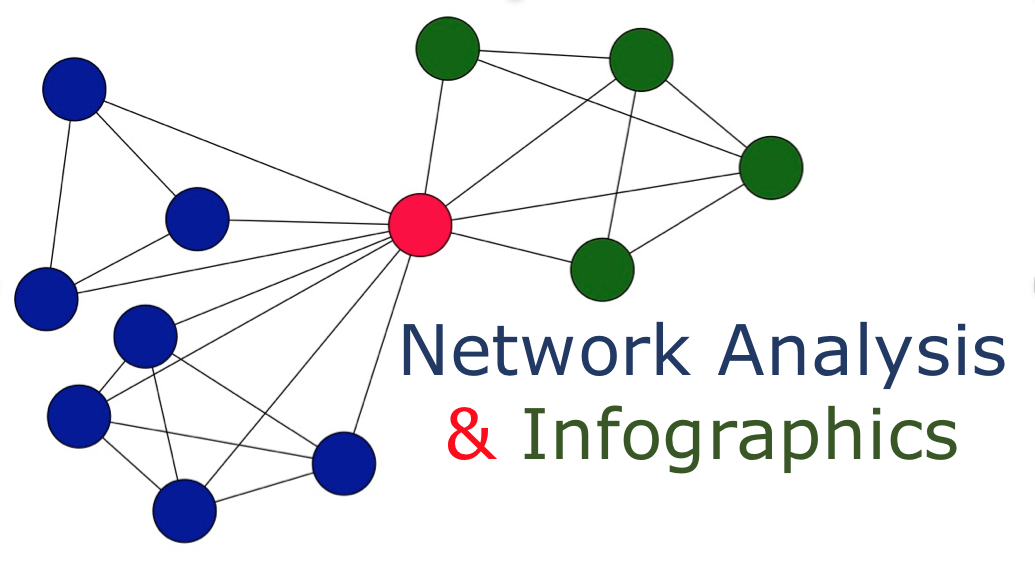
\includegraphics[width=2.5cm]{../_shared_pics/logo}

\medskip

\textit{{\color{dkgreen}{Week 3}}}\\
}


\date{} % Date, can be changed to a custom date

\begin{document}

\begin{frame}
\titlepage % Print the title page as the first slide

\begin{textblock*}{10pt}(0pt, 0.9\textheight)

\includegraphics[width=4cm]{../_shared_pics/SPRU.png}
\end{textblock*}

\end{frame}


%=======================================================
%	Learning outcomes
%=======================================================

\begin{frame}
\frametitle{Learning Outcomes}

\centering
\footnotesize
\begin{tabular}{lp{5.5cm}l}
\toprule
\multicolumn{2}{l}{\textbf{Learning outcome}} & \textbf{Assessment mode}\\
\hline
\\
1 & 
Explain the concept of network and list the main network indicators & 
ESS\\
\\
\rowcolor{green!20}2 & 
Describe and apply the major techniques for the collection of network data and their statistical analysis & 
ESS, GPN + GWS\\
\\
3 & 
Identify the main characteristics of networks by means of network measures  & 
ESS, GPN + GWS\\
\\
4 &
Employ network analysis techniques to produce network data-based infographics & 
GPN + GWS\\
\\
\bottomrule
\multicolumn{3}{l}{Note: ESS: Essay; GPN: Group Presentation; GWS: Group Written Submission}\\
\end{tabular}

\end{frame}

%------------------------------------------------




%=======================================================
%	Intro slides
%=======================================================

\begin{frame}
\frametitle{Overview}
\tableofcontents[hideallsubsections]
\end{frame}

%------------------------------------------------





%=======================================================
%	Defining a network (recap)
%=======================================================
\section*{Defining a network [recap]}
%------------------------------------------------

\bgroup
\setbeamercolor{background canvas}{bg = navyblue}
\begin{frame}[plain]{}
\begin{center}
\color{white}{\Huge\insertsection}
\end{center}
\end{frame}
\egroup

%------------------------------------------------

\begin{frame}
\frametitle{\insertsection}

\begin{columns}[c]
\column{.45\textwidth} 
	\begin{itemize}
	\item A {\color{blue}{graph}} is defined as:
	\end{itemize}

    \centering
	$G(N, E)$
    or
    $G(V, E, \phi)$

	\begin{itemize}
		\item $N$ nodes (or vertices), $N = {n_1, n_2, ..., n_N}$
		\item $E$ edges (or links, ties), $E = {e_1, e_2, ..., e_E}$
		\item Example: $G(7,8)$
		\item ``A network consists of {\color{blue}{a graph and additional information}} on the vertices or the lines of the graphs'' \citep{deNooy2005}
		
	\end{itemize}

\column{.45\textwidth}
\centering
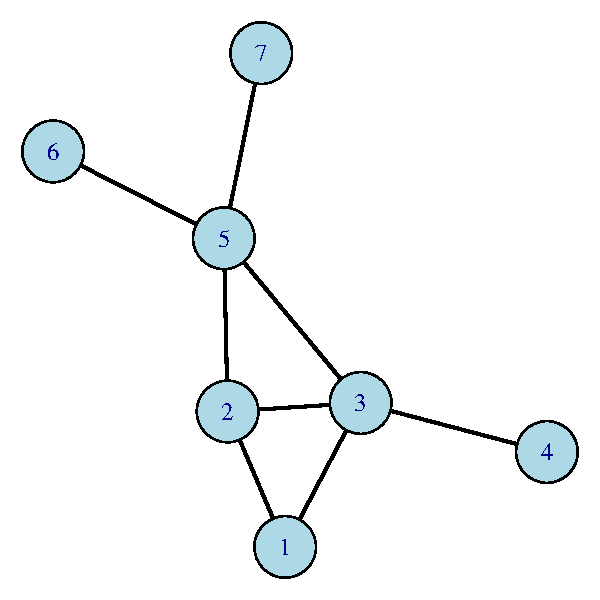
\includegraphics[width=5cm]{base}
\end{columns}

\end{frame}

%------------------------------------------------

\begin{frame}
\frametitle{\insertsection}

\begin{columns}[c]
\column{.45\textwidth} 
    \begin{itemize}
    \item {\color{blue}{Tie directionality}}: Undirected vs.\ directed networks
	\item {\color{blue}{Tie value}}: Unweighted vs.\ weighted networks
    \item {\color{blue}{Adjacency matrix}}: The (symmetric or asymmetric) matrix representing the connections among nodes 

    \item {\color{blue}{Definitions}}
    	\begin{itemize}  
    	\item Dyad, triad
    	\item Subgraph: line- or node-generated
    	\item Walk, trail, tour, path, shortest path (and geodesic distance)
    	\end{itemize}

    \item {\color{blue}{Types of networks}}
    	\begin{itemize}
    	\item Bipartite/2-mode networks
    	\item Multiplex/Multigraph networks
    	\item Ego-networks
   	 	\end{itemize}
	\end{itemize}

\column{.45\textwidth}
\centering
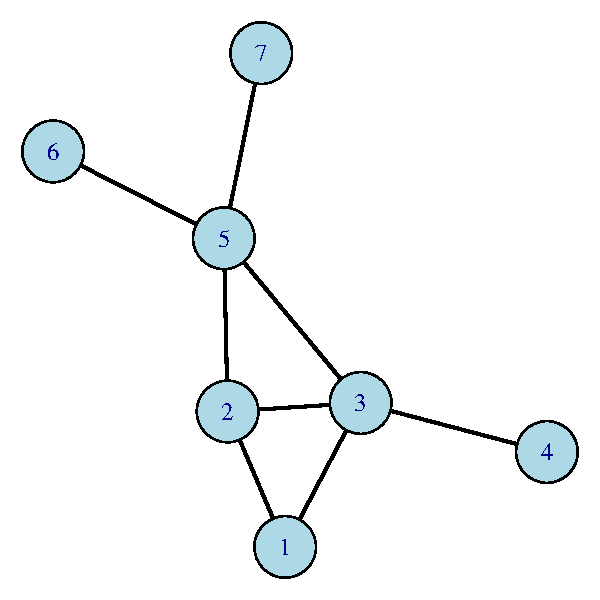
\includegraphics[width=5cm]{base}
\[\mathbf{A} =\left(\begin{array}{@{}cccc@{}}
             a_{11}&a_{12}&\cdots &a_{1N} \\
             a_{21}&a_{22}&\cdots &a_{2N} \\
             \vdots & \vdots & a_{ij} & \vdots\\
             a_{N1}&a_{N2}&\cdots &a_{NN}
             \end{array}\right)\]

\end{columns}

\end{frame}

%------------------------------------------------





%=======================================================
%	Data structure
%=======================================================
\section{Data structure}
%------------------------------------------------

\bgroup
\setbeamercolor{background canvas}{bg = navyblue}
\begin{frame}[plain]{}
\begin{center}
\color{white}{\Huge\insertsection}
\end{center}
\end{frame}
\egroup

%------------------------------------------------

\begin{frame}
\frametitle{\insertsection}
\framesubtitle{Variable analysis}

\footnotesize
\centering
\begin{tabular}{ccccc}
\multicolumn{5}{c}{Composition variables ({\color{blue}{attributes}})}\\
\toprule
Case & Variable $1$ & Variable $2$ & $\cdots$ & Variable $K$\\
\hline
$1$           \\
$2$           \\
$\vdots$      \\
$N$           \\
\bottomrule
\end{tabular}

\end{frame}

%------------------------------------------------

\begin{frame}[fragile]
\frametitle{\insertsection}
\framesubtitle{Variable analysis: Example}

\begin{columns}[c]

\column{.4\textwidth}
\begin{minipage}[c][.5\textheight][c]{\linewidth}

The {\color{blue}{Orange}} dataset includes data on the growth of orange trees
\begin{itemize}
\item 35 observations (5 trees)
\item 3 variables
\end{itemize}

\medskip
\medskip

\lstinputlisting[language=R, firstline=15, lastline=18]{handouts_script/L3_script_handouts.R}
\end{minipage}	   


\column{.6\textwidth}
\begin{minipage}[c][.5\textheight][c]{\linewidth}
\centering
\only<1>{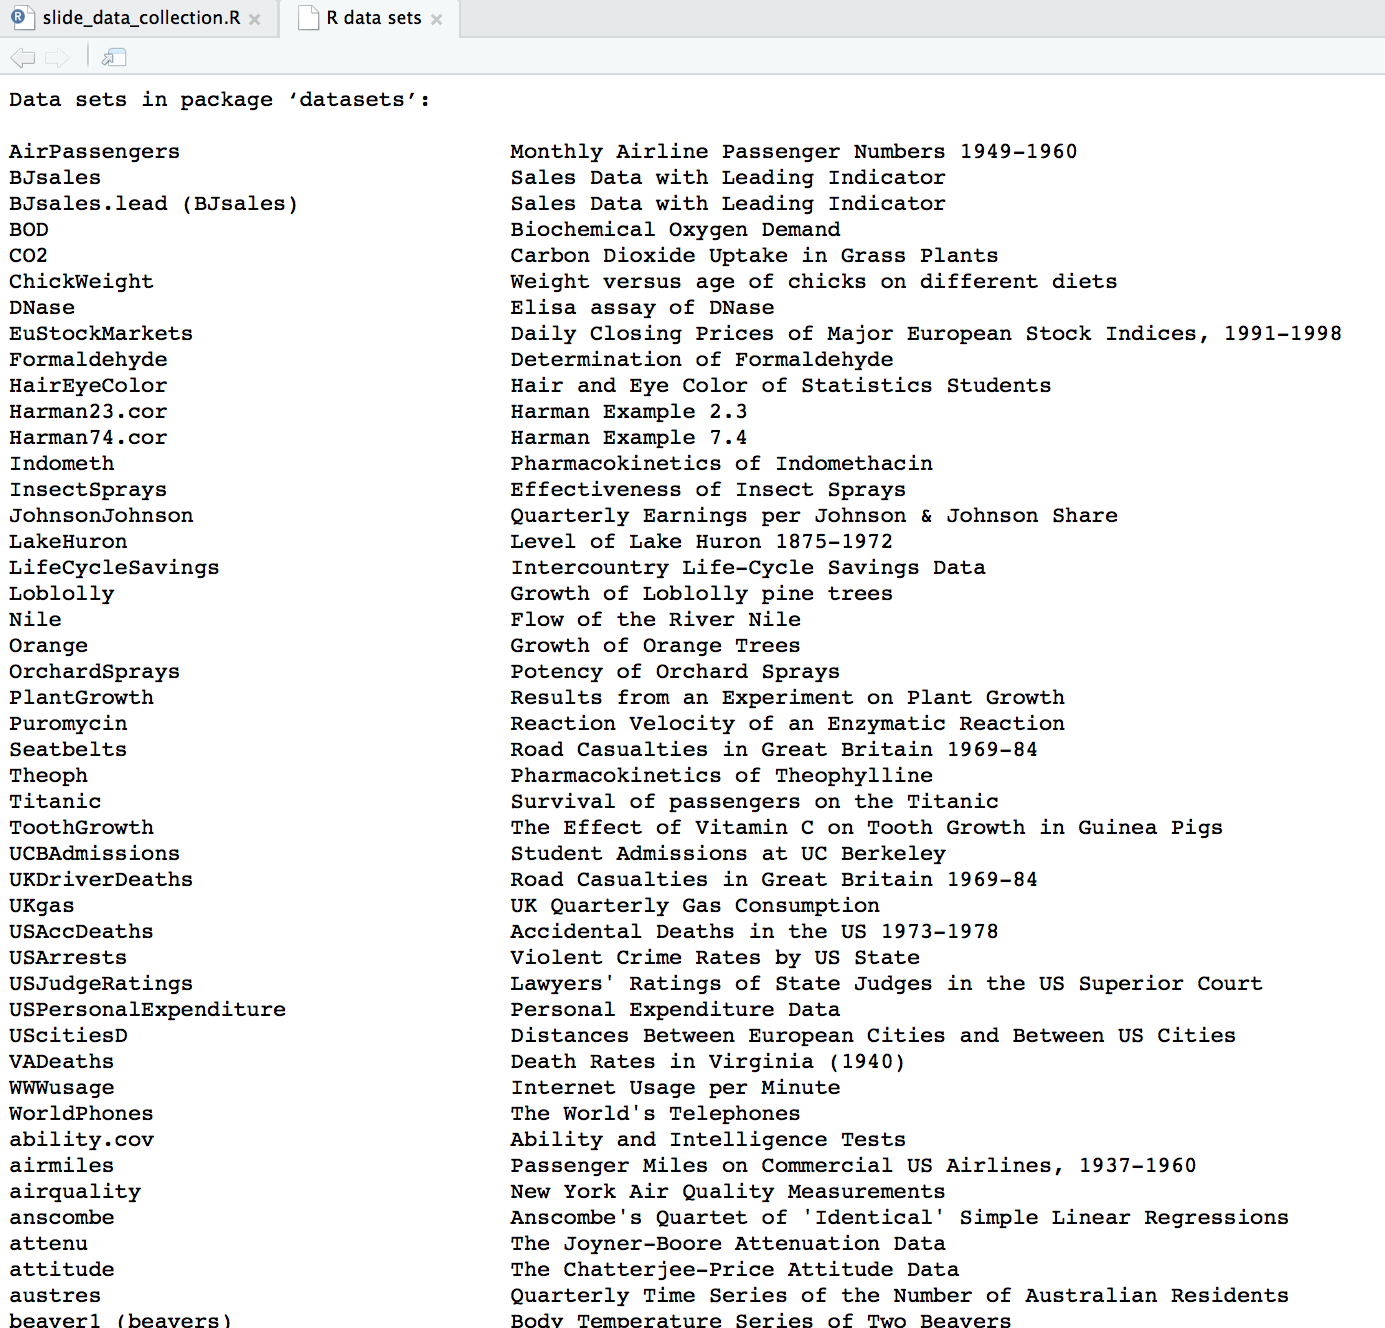
\includegraphics[width = 0.9\textwidth, frame]{dataR}}
\only<2>{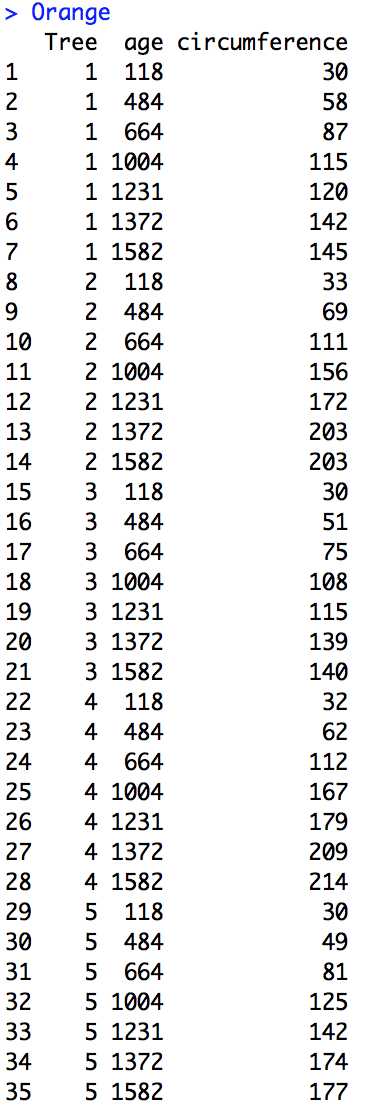
\includegraphics[height= 0.8\textheight]{orange_data}}
\only<3>{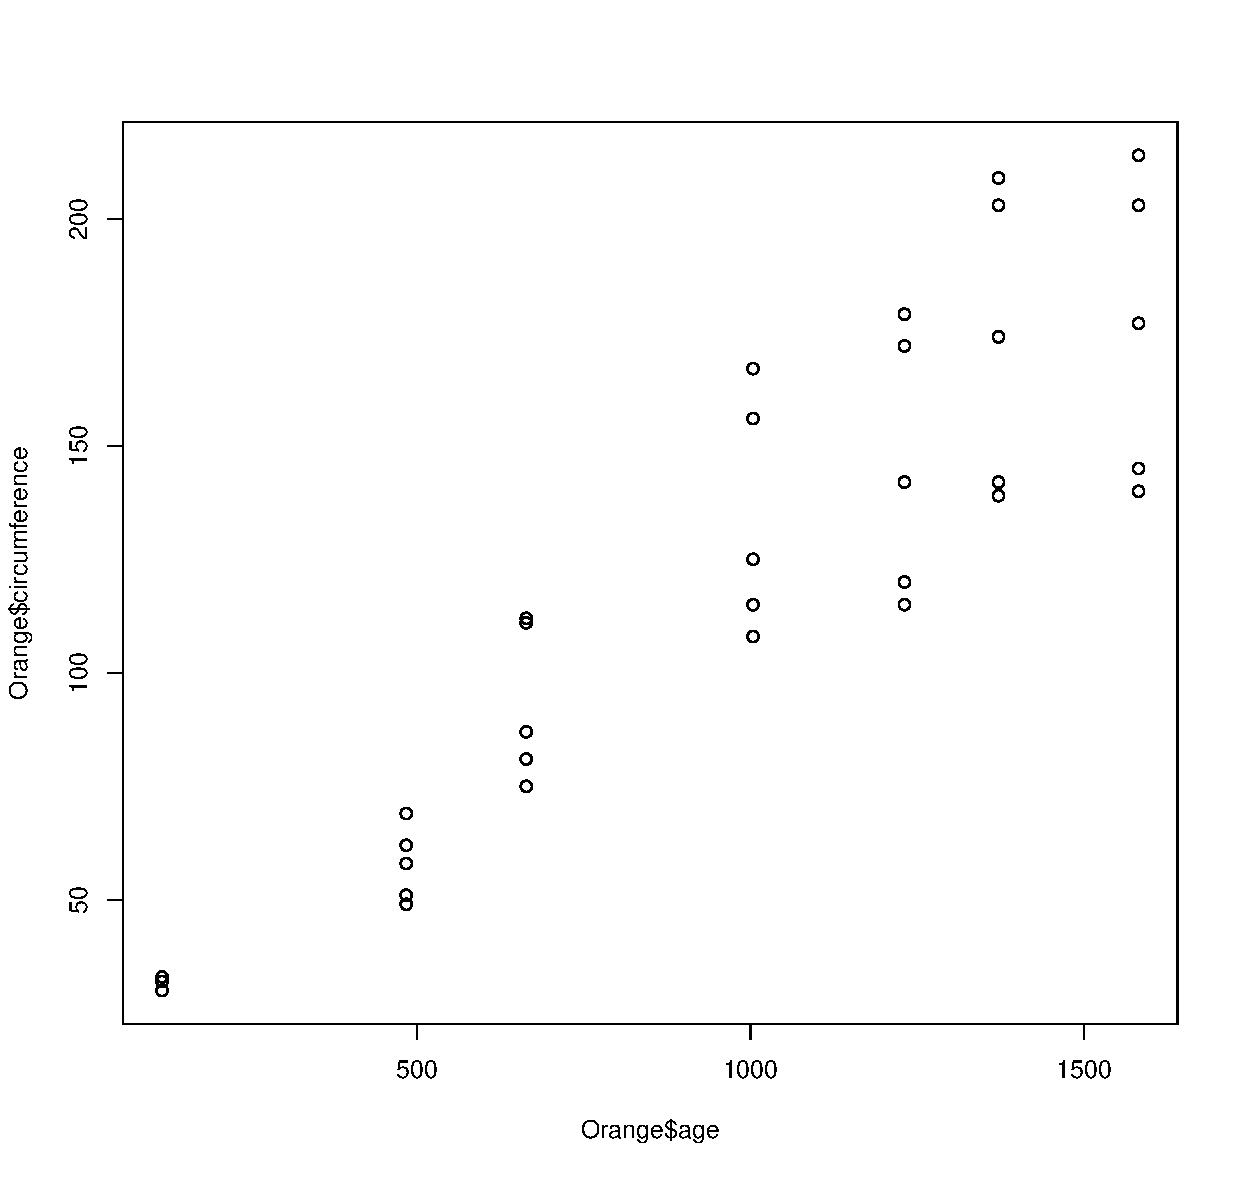
\includegraphics[width = 0.9\textwidth]{orange_plot}}
\end{minipage}

\end{columns}


\end{frame}



%------------------------------------------------


\begin{frame}
\frametitle{\insertsection}
\framesubtitle{Network analysis}

\footnotesize
\centering
\begin{tabular}{ccccc}
\multicolumn{5}{c}{Composition variables ({\color{blue}{attributes}})}\\
\toprule
Case & Variable $1$ & Variable $2$ & $\cdots$ & Variable $K$\\
\hline
$1$           \\
$2$           \\
$\vdots$      \\
$N$           \\
\bottomrule
\end{tabular}

\medskip
\medskip
\medskip
\medskip

\onslide<2>{
\footnotesize
\centering
\begin{tabular}{lcccccc}
\multicolumn{7}{c}{Structural variables ({\color{blue}{adjacency matrix}})}\\
\toprule
 &                & \multicolumn{4}{c}{Case}\\
        &        & $1$ & $2$ & $\cdots$ & $N$\\
\hline
        &    $1$           \\
        &    $2$           \\
Case    &    $\vdots$      \\
        &    $N$           \\
\bottomrule
\end{tabular}}


\end{frame}

%------------------------------------------------

\begin{frame}[fragile]
\frametitle{\insertsection}
\framesubtitle{Network analysis: Example}


\begin{columns}[c]

\column{.4\textwidth}
\begin{minipage}[c][.5\textheight][c]{\linewidth}


{\color{blue}{UKfaculty}} data on personal friendship in a UK faculty
\begin{itemize}
\item 81 individuals
\item 817 directed and weighted connections
\item Affiliation of each individual
\end{itemize}

\medskip
\medskip

\lstinputlisting[language=R, firstline=22, lastline=31]{handouts_script/L3_script_handouts.R}
\end{minipage}	   


\column{.6\textwidth}
\begin{minipage}[c][.5\textheight][c]{\linewidth}
\centering
\only<2>{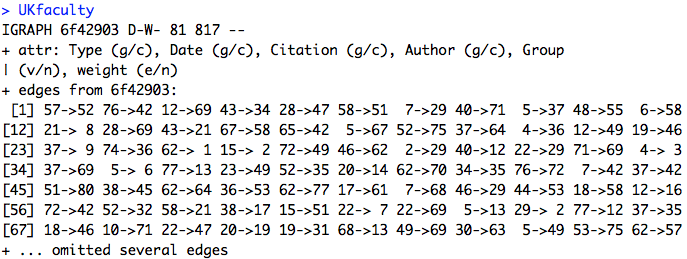
\includegraphics[width = 0.9\textwidth]{ukfaculty_data}}
\only<3>{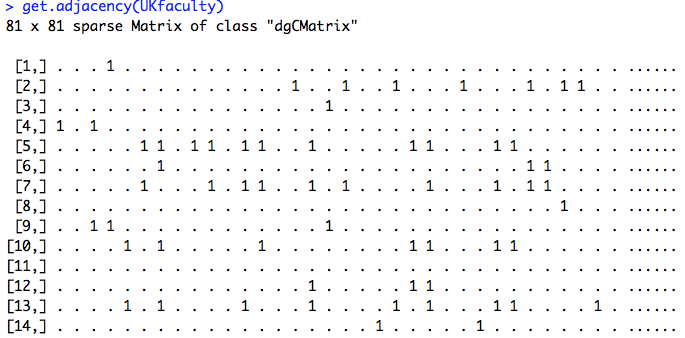
\includegraphics[width = 0.9\textwidth]{ukfaculty_adj}}
\only<4>{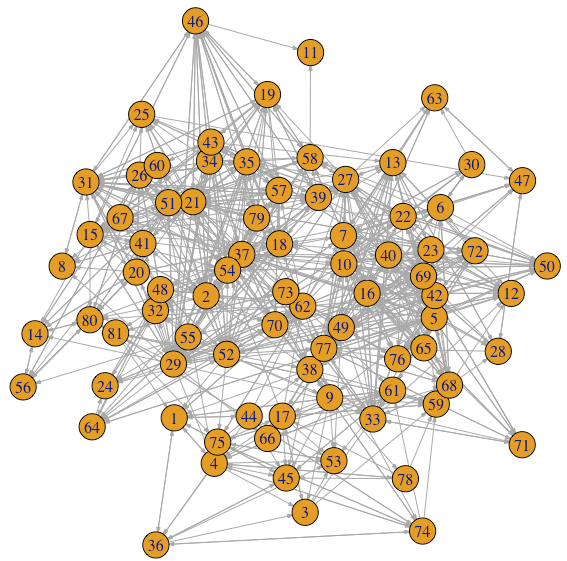
\includegraphics[width = 0.9\textwidth]{ukfaculty_plot}}
\end{minipage}

\end{columns}


\end{frame}

%------------------------------------------------

\begin{frame}[fragile]
\frametitle{\insertsection}
\framesubtitle{Network analysis: Network data}


\begin{columns}[c]

\column{.4\textwidth}
\begin{minipage}[c][.5\textheight][c]{\linewidth}

\begin{itemize}
\item Network data are structured as case-case tables: {\color{blue}{matrices or lists}} 
\item Such a format represents ties between cases (i.e.\ nodes)
\item These data are somewhat ready to be analysed
\end{itemize}

\end{minipage}	   


\column{.6\textwidth}
\begin{minipage}[c][.5\textheight][c]{\linewidth}

\footnotesize
\centering
\begin{tabular}{lccccc}
\multicolumn{6}{c}{Case-case {\color{blue}{adjacency matrix}}}\\
\toprule
        &        &\multicolumn{4}{c}{Case}\\
 
        &        & $1$ & $2$ & $\cdots$ & $N$\\
\hline
        &    $1$           \\
        &    $2$           \\
Case    &    $\vdots$      \\
        &    $N$           \\
\bottomrule
\end{tabular}


\medskip
\medskip
\medskip

\begin{tabular}{cc}
\multicolumn{2}{c}{Case-case {\color{blue}{list}}}\\
\toprule
Case  & Case\\
\hline
$1$           & $2$          \\
$2$           & $3$    \\
$\vdots$      & $\vdots$    \\
$i$           & $j$    \\
$\vdots$      & $\vdots$    \\
\bottomrule
\multicolumn{2}{l}{\tiny $i, j = \{1, 2, \cdots, N\}$}\\
\multicolumn{2}{l}{\tiny $i \ne j$}
\end{tabular}


\end{minipage}

\end{columns}


\end{frame}

%------------------------------------------------


\begin{frame}[fragile]
\frametitle{\insertsection}
\framesubtitle{Network analysis: Affiliation networks}


\begin{columns}[c]

\column{.4\textwidth}
\begin{minipage}[c][.5\textheight][c]{\linewidth}

\begin{itemize}[<+->]
\item Data are often available in the form of {\color{blue}{affiliation networks}} 
\item Such a format describes {\color{blue}{2-mode networks}}: individual-event, organization-R\&D alliance, researcher-publication, etc.
\item We need to transform these data before we can analyse them
\end{itemize}

\end{minipage}	   


\column{.6\textwidth}
\begin{minipage}[c][.5\textheight][c]{\linewidth}

\footnotesize
\centering
\begin{tabular}{lccccc}
\multicolumn{6}{c}{Case-affiliation {\color{blue}{adjacency matrix}}}\\
\toprule
        &        &\multicolumn{4}{c}{Affiliation}\\
 
        &        & $1$ & $2$ & $\cdots$ & $K$\\
\hline
        &    $1$           \\
        &    $2$           \\
Case    &    $\vdots$      \\
        &    $N$           \\
\bottomrule
\end{tabular}


\medskip
\medskip
\medskip

\begin{tabular}{cc}
\multicolumn{2}{c}{Case-affiliation {\color{blue}{list}}}\\
\toprule
Case  & Affiliation\\
\hline
$1$           & $2$          \\
$2$           & $3$    \\
$\vdots$      & $\vdots$    \\
$n$           & $k$    \\
$\vdots$      & $\vdots$    \\
\bottomrule
\multicolumn{2}{l}{\tiny $n = \{1, 2, \cdots, N\}$}\\
\multicolumn{2}{l}{\tiny $k = \{1, 2, \cdots, K\}$}\\
\end{tabular}


\end{minipage}

\end{columns}


\end{frame}

%------------------------------------------------

\begin{frame}
\frametitle{\insertsection}
\framesubtitle{Network analysis: Affiliation networks}


\centering
\footnotesize
\centering
\begin{tabular}{lccccc}
\multicolumn{6}{c}{Case-affiliation {\color{blue}{adjacency matrix}}}\\
\toprule
        &        &\multicolumn{4}{c}{Affiliation}\\
 
        &        & $1$ & $2$ & $\cdots$ & $K$\\
\hline
        &    $1$           \\
        &    $2$           \\
Case    &    $\vdots$      \\
        &    $N$           \\
\bottomrule
\end{tabular}


\medskip
\medskip
\medskip
\medskip

\begin{columns}[c]
\column{.45\textwidth} 
\footnotesize
\centering
\onslide<2->{\begin{tabular}{lccccc}
\multicolumn{6}{c}{(1)}\\
\\
\multicolumn{6}{c}{Case-case adjacency matrix}\\
\toprule
        &        &\multicolumn{4}{c}{Case}\\
 
        &        & $1$ & $2$ & $\cdots$ & $N$\\
\hline
        &    $1$           \\
        &    $2$           \\
Case    &    $\vdots$      \\
        &    $N$           \\
\bottomrule
\end{tabular}}


\column{.45\textwidth}
\footnotesize
\centering
\onslide<3->{\begin{tabular}{lccccc}
\multicolumn{6}{c}{(2)}\\
\\
\multicolumn{6}{c}{Affiliation-Affiliation adjacency matrix}\\
\toprule
        &        &\multicolumn{4}{c}{Affiliation}\\
 
        &        & $1$ & $2$ & $\cdots$ & $K$\\
\hline
        &    $1$           \\
        &    $2$           \\
Affiliation    &    $\vdots$      \\
        &    $K$           \\
\bottomrule
\end{tabular}}

\end{columns}


\end{frame}

%------------------------------------------------

\begin{frame}[fragile]
\frametitle{\insertsection}
\framesubtitle{Network analysis: Affiliation networks (example)}

\begin{columns}[c]

\column{.4\textwidth}
\begin{minipage}[c][.5\textheight][c]{\linewidth}


{\color{blue}{R\&D projects}} data
\begin{itemize}
\item 20 projects
\item 21 orgnisations
\end{itemize}

\medskip
\medskip

\onslide<5>{\lstinputlisting[language=R, firstline=35, lastline=44]{handouts_script/L3_script_handouts.R}}
\end{minipage}	   


\column{.6\textwidth}
\begin{minipage}[c][.5\textheight][c]{\linewidth}
\centering
\only<1>{
\centering
\scriptsize
\begin{table}
\begin{tabular}{clc}
\bottomrule
Project & Partners & Technology \\
\hline
Proj01          & U2, F1, NG1      & TechA      \\
Proj02          & U1, NG4, F1      & TechB      \\
Proj03          & NG3, NG1, F1     & TechC      \\
Proj04          & NG3, NG4, F1     & TechB      \\
Proj05          & U3, F1           & TechB      \\
Proj06          & U3, F2           & TechB      \\
Proj07          & U3, F3           & TechC      \\
Proj08          & U3, U4           & TechA      \\
Proj09          & F1               & TechB      \\
Proj10          & U5               & TechB      \\
Proj11          & U4, U5, U6       & TechA      \\
Proj12          & U3, U7           & TechB      \\
Proj13          & U7, G1           & TechB      \\
Proj14          & U7, O1           & TechD      \\
Proj15          & U7, G2           & TechD      \\
Proj16          & G2, F3           & TechC      \\
Proj17          & F3, O2           & TechC      \\
Proj18          & O2, F4, NG2      & TechB      \\
Proj19          & F4, U9, NG2      & TechB      \\
Proj20          & NG2, U8          & TechB		\\
\bottomrule     
\end{tabular}
\end{table}
}


\only<2>{
\centering
\footnotesize{(1) Transforming the table into long format}

\scriptsize
\begin{table}
\begin{tabular}{clc}
\bottomrule
Project & Partners & Technology \\
\hline
Proj01     & U2       & TechA     \\
Proj01     & F1       & TechA     \\
Proj01     & NG1      & TechA     \\
Proj02     & U1       & TechB     \\
Proj02     & NG4      & TechB     \\
Proj02     & F1       & TechB     \\
Proj03     & NG3      & TechC     \\
Proj03     & NG1      & TechC     \\
Proj03     & F1       & TechC     \\
Proj04     & NG3      & TechB     \\
Proj04     & NG4      & TechB     \\
Proj04     & F1       & TechB     \\
$\cdots$& $\cdots$ & $\cdots$     \\
Proj17    & F3       & TechC      \\
Proj17    & O2       & TechC      \\
Proj18    & O2       & TechB      \\
Proj18    & F4       & TechB      \\
Proj18    & NG2      & TechB      \\
Proj19    & F4       & TechB      \\
Proj19    & U9       & TechB      \\
Proj19    & NG2      & TechB      \\
Proj20    & NG2      & TechB      \\
Proj20    & U8       & TechB      \\
\bottomrule     
\end{tabular}
\end{table}}



\only<3>{
\centering
\footnotesize{(2) Co-occurence matrix}

\tiny
\setlength{\tabcolsep}{1pt}
\begin{table}
\begin{tabular}{c|ccccccccccccccccccccc}
\bottomrule
&	F1 & F2 & F3 & F4 & G1 & G2 & NG1 & NG2 & NG3 & NG4 & O1 & O2 & U1 & U2 & U3 & U4 & U5 & U6 & U7 & U8 & U9\\
\hline
Proj01 & 1  & 0  & 0  & 0  & 0  & 0   & 1   & 0   & 0   & 0  & 0  & 0  & 0  & 1  & 0  & 0  & 0  & 0  & 0  & 0  & 0 \\
Proj02 & 1  & 0  & 0  & 0  & 0  & 0   & 0   & 0   & 0   & 1  & 0  & 0  & 1  & 0  & 0  & 0  & 0  & 0  & 0  & 0  & 0 \\
Proj03 & 1  & 0  & 0  & 0  & 0  & 0   & 1   & 0   & 1   & 0  & 0  & 0  & 0  & 0  & 0  & 0  & 0  & 0  & 0  & 0  & 0 \\
Proj04 & 1  & 0  & 0  & 0  & 0  & 0   & 0   & 0   & 1   & 1  & 0  & 0  & 0  & 0  & 0  & 0  & 0  & 0  & 0  & 0  & 0 \\
Proj05 & 1  & 0  & 0  & 0  & 0  & 0   & 0   & 0   & 0   & 0  & 0  & 0  & 0  & 0  & 1  & 0  & 0  & 0  & 0  & 0  & 0 \\
Proj06 & 0  & 1  & 0  & 0  & 0  & 0   & 0   & 0   & 0   & 0  & 0  & 0  & 0  & 0  & 1  & 0  & 0  & 0  & 0  & 0  & 0 \\
Proj07 & 0  & 0  & 1  & 0  & 0  & 0   & 0   & 0   & 0   & 0  & 0  & 0  & 0  & 0  & 1  & 0  & 0  & 0  & 0  & 0  & 0 \\
Proj08 & 0  & 0  & 0  & 0  & 0  & 0   & 0   & 0   & 0   & 0  & 0  & 0  & 0  & 0  & 1  & 1  & 0  & 0  & 0  & 0  & 0 \\
Proj09 & 1  & 0  & 0  & 0  & 0  & 0   & 0   & 0   & 0   & 0  & 0  & 0  & 0  & 0  & 0  & 0  & 0  & 0  & 0  & 0  & 0 \\
Proj10 & 0  & 0  & 0  & 0  & 0  & 0   & 0   & 0   & 0   & 0  & 0  & 0  & 0  & 0  & 0  & 0  & 1  & 0  & 0  & 0  & 0 \\
Proj11 & 0  & 0  & 0  & 0  & 0  & 0   & 0   & 0   & 0   & 0  & 0  & 0  & 0  & 0  & 0  & 1  & 1  & 1  & 0  & 0  & 0 \\
Proj12 & 0  & 0  & 0  & 0  & 0  & 0   & 0   & 0   & 0   & 0  & 0  & 0  & 0  & 0  & 1  & 0  & 0  & 0  & 1  & 0  & 0 \\
Proj13 & 0  & 0  & 0  & 0  & 1  & 0   & 0   & 0   & 0   & 0  & 0  & 0  & 0  & 0  & 0  & 0  & 0  & 0  & 1  & 0  & 0 \\
Proj14 & 0  & 0  & 0  & 0  & 0  & 0   & 0   & 0   & 0   & 0  & 1  & 0  & 0  & 0  & 0  & 0  & 0  & 0  & 1  & 0  & 0 \\
Proj15 & 0  & 0  & 0  & 0  & 0  & 1   & 0   & 0   & 0   & 0  & 0  & 0  & 0  & 0  & 0  & 0  & 0  & 0  & 1  & 0  & 0 \\
Proj16 & 0  & 0  & 1  & 0  & 0  & 1   & 0   & 0   & 0   & 0  & 0  & 0  & 0  & 0  & 0  & 0  & 0  & 0  & 0  & 0  & 0 \\
Proj17 & 0  & 0  & 1  & 0  & 0  & 0   & 0   & 0   & 0   & 0  & 0  & 1  & 0  & 0  & 0  & 0  & 0  & 0  & 0  & 0  & 0 \\
Proj18 & 0  & 0  & 0  & 1  & 0  & 0   & 0   & 1   & 0   & 0  & 0  & 1  & 0  & 0  & 0  & 0  & 0  & 0  & 0  & 0  & 0 \\
Proj19 & 0  & 0  & 0  & 1  & 0  & 0   & 0   & 1   & 0   & 0  & 0  & 0  & 0  & 0  & 0  & 0  & 0  & 0  & 0  & 0  & 1\\
\bottomrule     
\end{tabular}
\end{table}
}




\only<4>{
\centering
\footnotesize{(3) Matrix product}

\tiny
\setlength{\tabcolsep}{1pt}
\begin{table}
\begin{tabular}{c|ccccccccccc}
\bottomrule
       &Proj01 & Proj02 & Proj03 & Proj04 & Proj05 & Proj06 & Proj07 & Proj08 & Proj09 & ... &   \\
\hline
F1     & 1      & 1      & 1      & 1      & 1      & 0      & 0      & 0      & 1      & ... \\
F2     & 0      & 0      & 0      & 0      & 0      & 1      & 0      & 0      & 0      & ... \\
F3     & 0      & 0      & 0      & 0      & 0      & 0      & 1      & 0      & 0      & ... \\
F4     & 0      & 0      & 0      & 0      & 0      & 0      & 0      & 0      & 0      & ... \\
G1     & 0      & 0      & 0      & 0      & 0      & 0      & 0      & 0      & 0      & ... \\
... &  ...  & ...  & ...  & ... & ... \\

\end{tabular}
\end{table}


X

\centering
\tiny
\setlength{\tabcolsep}{1pt}
\begin{table}
\begin{tabular}{c|ccccccc}
\bottomrule
	   &F1  & F2 & F3 & F4 & G1 & ...   \\
\hline
Proj01 & 1  & 0  & 0  & 0  & 0 & ...\\
Proj02 & 1  & 0  & 0  & 0  & 0 & ...\\
Proj03 & 1  & 0  & 0  & 0  & 0 & ...\\
Proj04 & 1  & 0  & 0  & 0  & 0 & ...\\
Proj05 & 1  & 0  & 0  & 0  & 0 & ...\\
Proj06 & 0  & 1  & 0  & 0  & 0 & ...\\
Proj07 & 0  & 0  & 1  & 0  & 0 & ...\\
Proj08 & 0  & 0  & 0  & 0  & 0 & ...\\
Proj09 & 1  & 0  & 0  & 0  & 0 & ...\\
... &  ...  & ...  & ...  & ... & ... \\
\end{tabular}
\end{table}

}





\only<5>{
\centering
\footnotesize{(4) Adjacency matrix}

\tiny
\setlength{\tabcolsep}{1pt}
\begin{table}
\begin{tabular}{c|ccccccccccccccccccccc}
\bottomrule
    & F1  & F2 & F3 & F4 & G1 & G2 & NG1 & NG2 & NG3 & NG4 & O1 & O2 & U1 & U2 & U3 & U4 & U5 & U6 & U7 & U8 & U9 \\
\hline
F1  & 0  & 0  & 0  & 0  & 0  & 0   & 2   & 0   & 2   & 2  & 0  & 0  & 1  & 1  & 1  & 0  & 0  & 0  & 0  & 0  & 0 \\
F2  & 0  & 0  & 0  & 0  & 0  & 0   & 0   & 0   & 0   & 0  & 0  & 0  & 0  & 0  & 1  & 0  & 0  & 0  & 0  & 0  & 0 \\
F3  & 0  & 0  & 0  & 0  & 0  & 1   & 0   & 0   & 0   & 0  & 0  & 1  & 0  & 0  & 1  & 0  & 0  & 0  & 0  & 0  & 0 \\
F4  & 0  & 0  & 0  & 0  & 0  & 0   & 0   & 2   & 0   & 0  & 0  & 1  & 0  & 0  & 0  & 0  & 0  & 0  & 0  & 0  & 1 \\
G1  & 0  & 0  & 0  & 0  & 0  & 0   & 0   & 0   & 0   & 0  & 0  & 0  & 0  & 0  & 0  & 0  & 0  & 0  & 1  & 0  & 0 \\
G2  & 0  & 0  & 1  & 0  & 0  & 0   & 0   & 0   & 0   & 0  & 0  & 0  & 0  & 0  & 0  & 0  & 0  & 0  & 1  & 0  & 0 \\
NG1 & 2  & 0  & 0  & 0  & 0  & 0   & 0   & 0   & 1   & 0  & 0  & 0  & 0  & 1  & 0  & 0  & 0  & 0  & 0  & 0  & 0 \\
NG2 & 0  & 0  & 0  & 2  & 0  & 0   & 0   & 0   & 0   & 0  & 0  & 1  & 0  & 0  & 0  & 0  & 0  & 0  & 0  & 1  & 1 \\
NG3 & 2  & 0  & 0  & 0  & 0  & 0   & 1   & 0   & 0   & 1  & 0  & 0  & 0  & 0  & 0  & 0  & 0  & 0  & 0  & 0  & 0 \\
NG4 & 2  & 0  & 0  & 0  & 0  & 0   & 0   & 0   & 1   & 0  & 0  & 0  & 1  & 0  & 0  & 0  & 0  & 0  & 0  & 0  & 0 \\
O1  & 0  & 0  & 0  & 0  & 0  & 0   & 0   & 0   & 0   & 0  & 0  & 0  & 0  & 0  & 0  & 0  & 0  & 0  & 1  & 0  & 0 \\
O2  & 0  & 0  & 1  & 1  & 0  & 0   & 0   & 1   & 0   & 0  & 0  & 0  & 0  & 0  & 0  & 0  & 0  & 0  & 0  & 0  & 0 \\
U1  & 1  & 0  & 0  & 0  & 0  & 0   & 0   & 0   & 0   & 1  & 0  & 0  & 0  & 0  & 0  & 0  & 0  & 0  & 0  & 0  & 0 \\
U2  & 1  & 0  & 0  & 0  & 0  & 0   & 1   & 0   & 0   & 0  & 0  & 0  & 0  & 0  & 0  & 0  & 0  & 0  & 0  & 0  & 0 \\
U3  & 1  & 1  & 1  & 0  & 0  & 0   & 0   & 0   & 0   & 0  & 0  & 0  & 0  & 0  & 0  & 1  & 0  & 0  & 1  & 0  & 0 \\
U4  & 0  & 0  & 0  & 0  & 0  & 0   & 0   & 0   & 0   & 0  & 0  & 0  & 0  & 0  & 1  & 0  & 1  & 1  & 0  & 0  & 0 \\
U5  & 0  & 0  & 0  & 0  & 0  & 0   & 0   & 0   & 0   & 0  & 0  & 0  & 0  & 0  & 0  & 1  & 0  & 1  & 0  & 0  & 0 \\
U6  & 0  & 0  & 0  & 0  & 0  & 0   & 0   & 0   & 0   & 0  & 0  & 0  & 0  & 0  & 0  & 1  & 1  & 0  & 0  & 0  & 0 \\
U7  & 0  & 0  & 0  & 0  & 1  & 1   & 0   & 0   & 0   & 0  & 1  & 0  & 0  & 0  & 1  & 0  & 0  & 0  & 0  & 0  & 0 \\
U8  & 0  & 0  & 0  & 0  & 0  & 0   & 0   & 1   & 0   & 0  & 0  & 0  & 0  & 0  & 0  & 0  & 0  & 0  & 0  & 0  & 0 \\
U9  & 0  & 0  & 0  & 1  & 0  & 0   & 0   & 1   & 0   & 0  & 0  & 0  & 0  & 0  & 0  & 0  & 0  & 0  & 0  & 0  & 0 \\
\bottomrule     
\end{tabular}
\end{table}
}

\end{minipage}

\end{columns}

\end{frame}

%------------------------------------------------





%=======================================================
%	Data collection
%=======================================================
\section{Data collection}

%------------------------------------------------

\bgroup
\setbeamercolor{background canvas}{bg = navyblue}
\begin{frame}[plain]{}
\begin{center}
\color{white}{\Huge\insertsection}
\end{center}
\end{frame}
\egroup

%------------------------------------------------

\begin{frame}
\frametitle{\insertsection}
\framesubtitle{Key questions}

\begin{columns}[c]
\column{.45\textwidth}

\begin{itemize}
\item Define a set of {\color{blue}{nodes}}
		\begin{itemize}
		\item Which actors should be included? 
		\item Which are the relevant actors for the network?
		\item Can we sample nodes/actors?
		\item ...
		\end{itemize}

\medskip

\item Define a set of {\color{blue}{ties}} between nodes
	\begin{itemize}
		\item Which relations should be included?
		\item Which relations are likely to be excluded?
		\item ...
		\end{itemize}	
\end{itemize}

		
		
\column{.45\textwidth}
\footnotesize
\centering
\begin{tabular}{lccccc}
\multicolumn{6}{c}{Case-case {\color{blue}{adjacency matrix}}}\\
\toprule
        &        &\multicolumn{4}{c}{Case}\\
 
        &        & $1$ & $2$ & $\cdots$ & $N$\\
\hline
        &    $1$           \\
        &    $2$           \\
Case    &    $\vdots$      \\
        &    $N$           \\
\bottomrule
\end{tabular}

\end{columns}


\end{frame}

%------------------------------------------------

\begin{frame}
\frametitle{\insertsection}
\framesubtitle{Defining the set of nodes}

In the case of relational data, {\color{blue}{we cannot independently sample actors}}
	\begin{itemize}
	\item If an actor is selected, {\color{blue}{all actors}} to whom the actor is connected should be included 
	\item Network studies tend to focus on {\color{blue}{whole populations/samples of convenience}}	
	\item We need to define the {\color{blue}{boundaries}} of our population/sample

		\begin{itemize}
		\item In some cases, we have some {\color{blue}{\textit{a priori} knowledge}} to identify the set of actors
			\begin{itemize}
			\item employees in a firm
			\item students in this module
			\item ...
			\end{itemize}
	
		\item In other cases, drawing boundaries around a set of nodes is somewhat {\color{blue}{arbitrary}}
			\begin{itemize}
			\item It may be difficult to understand whether a {\color{blue}{an actor belongs to the set}}
			\item The population may be too {\color{blue}{large}}
			\item The composition of actors may change over time ({\color{blue}{joiners and leavers}})
			\end{itemize}
		\end{itemize}
	
	\end{itemize}

\end{frame}

%------------------------------------------------

\begin{frame}
\frametitle{\insertsection}
\framesubtitle{Defining the set of nodes}


\citet{Laumann1989} and the {\color{blue}{'boundary specification problem'}}
		
	\begin{itemize}[<+(1)->]
	\item {\color{blue}{Realist approach:}} focus on actors to identify network boundaries as perceived by the actors themselves\\		
		
		\medskip
		
		\textit{Example\\
		With whom you discuss important study related matters?\\
		Focus on a class/course may leave network ties outside the study}
		
		\medskip
		
	\item {\color{blue}{Nominalist approach:}} focus on the theoretical concerns of the researcher/analyst\\
		
		\medskip
		
		\textit{Example\\
		How does degree centrality affect scientists' productivity in cancer research?\\
		Focus on a researchers that published in cancer}
	
	\end{itemize}
\centering
		
\medskip
	
\onslide<4>{{\color{red}{The research question guides the selection of the approach}}}


\end{frame}


%------------------------------------------------

\begin{frame}
\frametitle{\insertsection}
\framesubtitle{Defining the set of ties}

Once we have identified a set of actors, we need to identify the corresponding  {\color{blue}{set of ties}} between these actors

\medskip

\begin{itemize}
\item {\color{blue}{Full-network method}}
\item {\color{blue}{Snowball method}}
\item {\color{blue}{Ego-centric method}}
\end{itemize}

\end{frame}

%------------------------------------------------

\begin{frame}
\frametitle{\insertsection}
\framesubtitle{Defining the set of ties}

{\color{blue}{Full-network method}}
\begin{itemize}
\item We collect information about each tie between the actors in our population/sample
\item This approach can generate a {\color{dkgreen}{comprehensive map}} of a network
\item Actors tend to establish a limited number of ties ({\color{blue}{limited attentional capabilities}})
\item Feasibility in the case of {\color{red}{relatively small networks}} -- time and resources to collect data  (e.g.\ ties between people living in a city)
\end{itemize}

\end{frame}

%------------------------------------------------

\begin{frame}
\frametitle{\insertsection}
\framesubtitle{Defining the set of ties}

\begin{columns}[c]
\column{.40\textwidth}
Example of {\color{blue}{full-network method}}
\begin{itemize}
\item Aim: To map medication advice-seeking interactions of doctors, nurses, allied health professionals 
\item Context: Renal ward of an Australian metropolitan teaching hospital
\item Data collection: Questionnaires with the full list of staff(response rate 96\%)
\end{itemize}

\column{.60\textwidth}
\centering
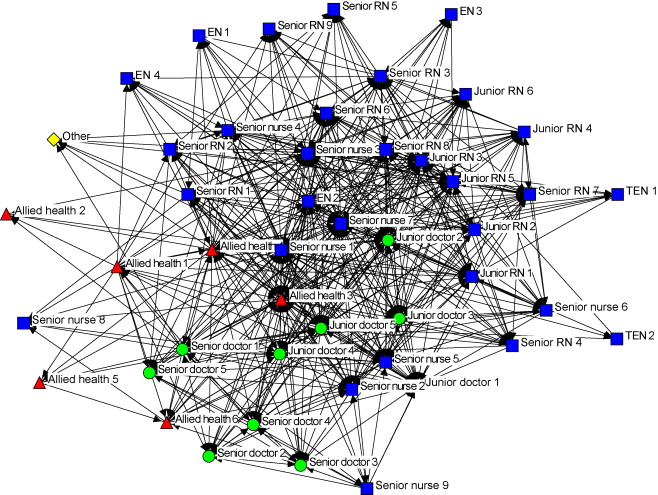
\includegraphics[width=\textwidth]{full_example.jpg}\\
\tiny{Source: \citet{Creswick2010}}

\end{columns}

\end{frame}

%Comments on the results of the paper
%On average, there is little interaction between each of the staff members in the medication advice-seeking network, with even less interaction between staff from different professional groups. Nurses are mainly located on one side of the network and doctors on the other. However, the pharmacist is quite central in the medication advice-seeking network as are some senior nurses and a junior doctor.

%------------------------------------------------

\begin{frame}
\frametitle{\insertsection}
\framesubtitle{Defining the set of ties}

{\color{blue}{Snowball method}}
\begin{itemize}
\item We ask to each actor in our set to list some or all of their ties with other actors
\item All the actors listed, but not included in the original set of actors are tracked down and asked for some or all of their ties
\item The process stops when
	\begin{itemize} 
	\item no new actors are identified
	\item the new actors are very `marginal' to the set of actors under study
	\item we have limitations of time and resources
	\end{itemize}
\item It is likely to require {\color{dkgreen}{less time and resources}} than the full-network approach	
\item {\color{red}{Isolated actors}} may not be captured (overestimation of network cohesion)
\item A wrong starting set of actors may {\color{red}{miss entire sub-sets of actors}} not linked to our starting set of actors (e.g.\ multiple components)
\end{itemize}
\end{frame}

%------------------------------------------------

\begin{frame}
\frametitle{\insertsection}
\framesubtitle{Defining the set of ties}

\centering
Example of {\color{blue}{snowball-network method}}

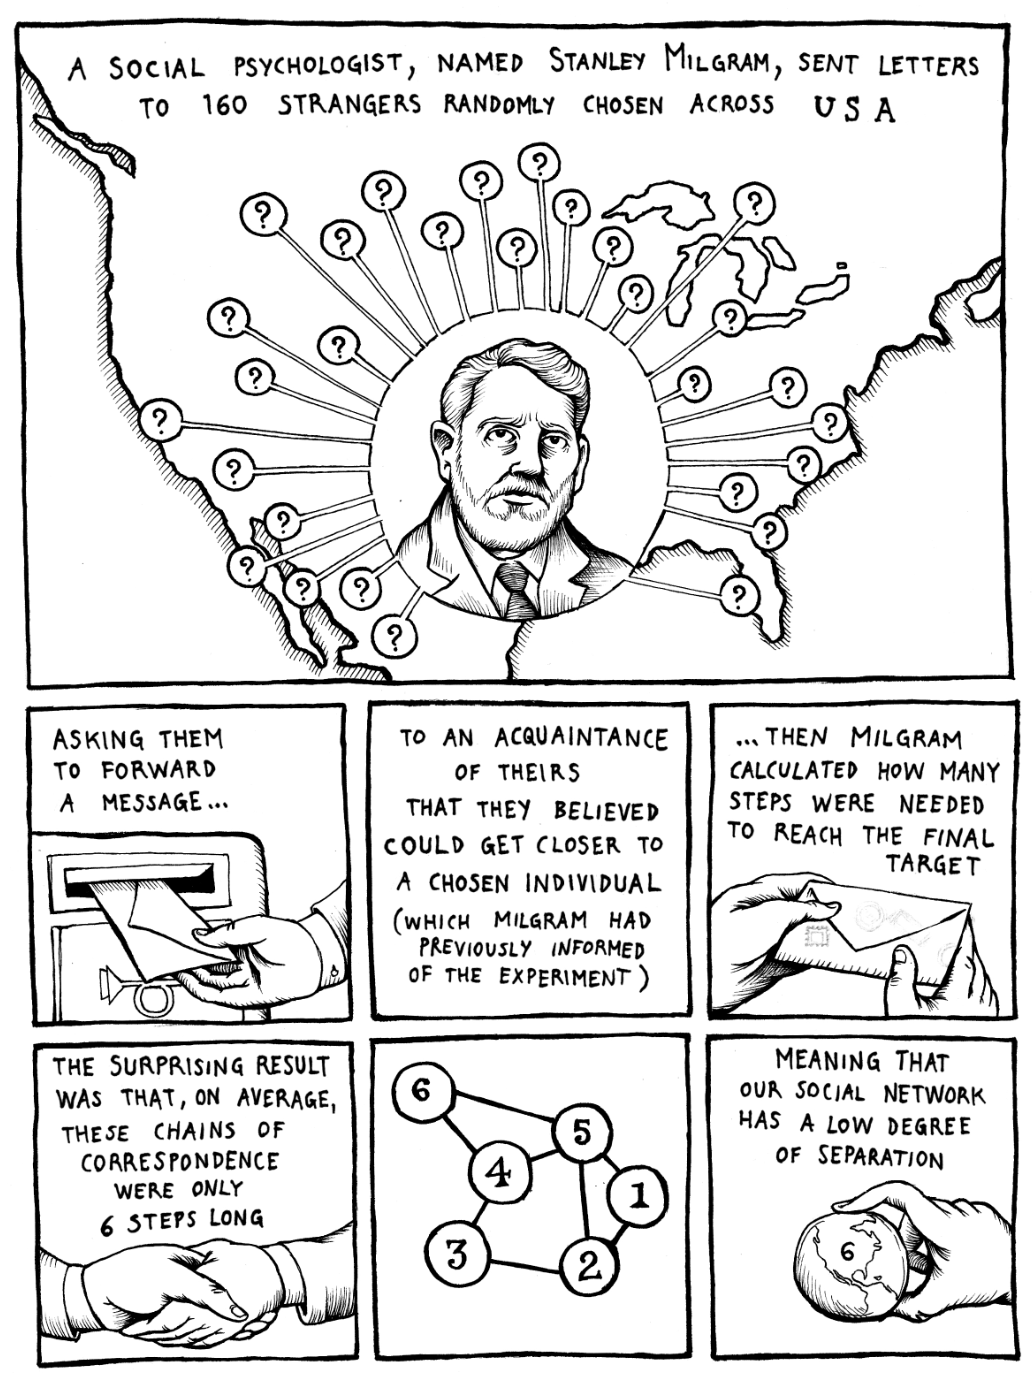
\includegraphics[width=0.4\textwidth]{milgram}\\
\tiny{Source: https://matteofarinella.wordpress.com/2010/09/05/a-small-world-theory/}\\
\tiny{Video: \url{https://youtu.be/NberyK6kt8c}}

\end{frame}

%------------------------------------------------


\begin{frame}
\frametitle{\insertsection}
\framesubtitle{Defining the set of ties}


\begin{columns}[c]
\column{.60\textwidth}
{\color{blue}{Ego-centric method}}
\begin{itemize}
\item  We start with a set of focal actors (egos), and identify the actors to which they are connected
\item Useful when we have {\color{dkgreen}{feasibility issues}} with other methods
\item We ask to the egos to report which of their direct peers are also tied to one another 
\item Relatively reliable overview of at least the {\color{dkgreen}{local neighbourhoods}} in which the selected actors are embedded (e.g.\ redundancy and constraint)
\item Not useful to estimate {\color{red}{network-level measures}}
\end{itemize}

\column{.40\textwidth}
\centering
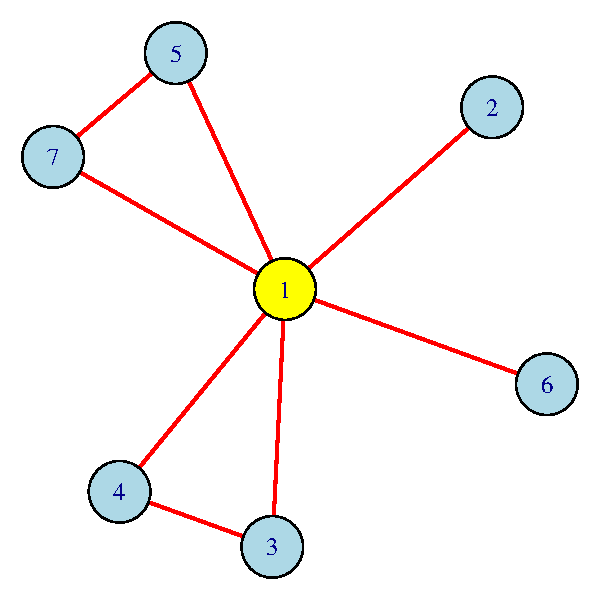
\includegraphics[width=4cm]{egomet}
\end{columns}

\end{frame}

%------------------------------------------------


%=======================================================
%	Data sources
%=======================================================
\section{Data sources}

%------------------------------------------------

\bgroup
\setbeamercolor{background canvas}{bg = navyblue}
\begin{frame}[plain]{}
\begin{center}
\color{white}{\Huge\insertsection}
\end{center}
\end{frame}
\egroup

%------------------------------------------------


\begin{frame}
\frametitle{\insertsection}

\begin{itemize}
\item Questionnaires (or surveys)
\item Interviews
\item Observations
\item Archival data
\end{itemize}

\end{frame}

%------------------------------------------------

\begin{frame}
\frametitle{\insertsection}
\framesubtitle{Questionnaires}

\begin{itemize}
\item Commonly used to map {\color{blue}{relatively small social networks}}
\item Respondents report their ties with other actors in the network 
    \begin{itemize}
    \item who they like
    \item who they seek advice from
    \item who they collaborate with
    \item ...
    \end{itemize}  
\item Three main choices
    \begin{itemize}
    \item {\color{blue}{Choice 1}}: predefined or undefined list of names 
    \item {\color{blue}{Choice 2}}: constraints on the number of ties
    \item {\color{blue}{Choice 3}}: value of the ties
    \end{itemize}

\end{itemize}

\end{frame}

%------------------------------------------------
\begin{frame}
\frametitle{\insertsection}
\framesubtitle{Questionnaires - Choice 1: Roster}

\begin{columns}[c]

\column{.45\textwidth}
\begin{itemize}
\item All the actors in a network are represented in a {\color{blue}{roster}}
\item Respondents indicate the existence of {\color{blue}{ ties}} with all the other actors in the network
\end{itemize} 


\column{.45\textwidth} 
\footnotesize
\centering
\begin{tabular}{lcc}
\multicolumn{3}{c}{\textbf{Roster}} \\
\toprule
\textbf{Name} & \textbf{Friend} & \textbf{Advice}\\
\hline
Peter Parker      &$\Box$    &$\Box$  \\
Tony Stark        &$\Box$    &$\Box$  \\
Bruce Banner      &$\Box$    &$\Box$  \\
...               &...       &...     \\
\bottomrule
\end{tabular}

\end{columns}


\end{frame}

%------------------------------------------------

\begin{frame}
\frametitle{\insertsection}
\framesubtitle{Questionnaires - Choice 1: Roster}

\begin{columns}[t]

\column{.45\textwidth}
{\color{dkgreen}{Advantages}}
\begin{itemize}
\item Respondents {\color{dkgreen}{recognise names}}
\item Minimum {\color{dkgreen}{data cleaning}} (name spelling)
\end{itemize} 

\column{.45\textwidth}
{\color{red}{Limitations}}
\begin{itemize}
\item Feasible for {\color{red}{small networks}}
\item Need of {\color{red}{well-delineated boundaries}}
    \begin{itemize}
    \item students in this module
    \item employees in a firms' department/business unit
    \item ...
    \end{itemize} 
\end{itemize} 

\end{columns}

\end{frame}

%------------------------------------------------

\begin{frame}
\frametitle{\insertsection}
\framesubtitle{Questionnaires - Choice 1: Free recall}

\begin{columns}[c]

\column{.45\textwidth}
\begin{itemize}
\item The {\color{blue}{list of names}} is generated by respondents
\item Respondents name the actors with which they have {\color{blue}{certain ties}}

\end{itemize} 


\column{.45\textwidth} 
\footnotesize
\centering
\begin{tabular}{lcc}
\multicolumn{3}{c}{\textbf{Free recall}} \\
\toprule
\textbf{Name} & \textbf{Friend} & \textbf{Advice}\\
\hline
\_\_\_\_\_\_\_\_\_        &$\Box$    &$\Box$  \\
\_\_\_\_\_\_\_\_\_        &$\Box$    &$\Box$  \\
\_\_\_\_\_\_\_\_\_        &$\Box$    &$\Box$  \\
\_\_\_\_\_\_\_\_\_        &$\Box$    &$\Box$  \\
...                		  &...       &...  \\
\bottomrule
\end{tabular}

\end{columns}

\end{frame}

%------------------------------------------------

\begin{frame}
\frametitle{\insertsection}
\framesubtitle{Questionnaires - Choice 1: Free recall}

\begin{columns}[t]

\column{.45\textwidth}
{\color{dkgreen}{Advantages}}
\begin{itemize}
\item Respondents can name actors not included in the {\color{dkgreen}{initial delineation of the network boundaries}} (snowball)
\item Useful when the {\color{dkgreen}{boundaries}} of the network are not clear
    \begin{itemize}
    \item friendship network in high school
    \item researchers working in a discipline
    \item ...
    \end{itemize}
\end{itemize}


\column{.45\textwidth}
{\color{red}{Limitations}}
\begin{itemize}
\item Respondents may be {\color{red}{unwilling or uncomfortable}} to name actors
\item {\color{red}{Data cleaning}} (name spelling)
\item Time and resources to {\color{red}{contact `snowballed' actors}}
\end{itemize}

\end{columns}

\end{frame}

%------------------------------------------------

\begin{frame}
\frametitle{\insertsection}
\framesubtitle{Questionnaires - Choice 2: Free vs.\ Fixed choice}

\begin{columns}[t]

\column{.45\textwidth}
{\color{blue}{Free choice}}
\begin{itemize}
\item Respondents have no constraints on the {\color{blue}{number of actors}} they can name
\item No constraints on the {\color{blue}{maximum number of ties}} of respondents' ego-network
\item \textit{Please identify people who you have exchanged ideas with most often ...}
\end{itemize} 


\column{.45\textwidth}
{\color{blue}{Fixed choice}}
\begin{itemize}
\item Respondents have constraints on the {\color{blue}{number of actors}} they can nominate
\item There is a {\color{blue}{maximum number of ties}} that each actor can have in the network
\item \textit{Please identify up to N people who you have exchanged ideas with most often ...}
\end{itemize} 

\end{columns}

\end{frame}

%------------------------------------------------

\begin{frame}
\frametitle{\insertsection}
\framesubtitle{Questionnaires - Choice 3: Rating vs.\ Ranking choice}

\begin{columns}[t]

\column{.45\textwidth}
{\color{blue}{Rating}}
\begin{itemize}
\item Respondents are asked to assign a {\color{blue}{value}} to each tie
\end{itemize} 


\column{.45\textwidth}
{\color{blue}{Complete ranking}}
\begin{itemize}
\item Respondents are asked to {\color{blue}{rank all their ties}}
\end{itemize} 

\end{columns}

\end{frame}

%------------------------------------------------

\begin{frame}
\frametitle{\insertsection}
\framesubtitle{Interviews}

\begin{itemize}
\item Face-to-face, over the phone, videoconferencing
\item Used when survey are not feasible (willing to participate)
\item Gather {\color{blue}{ego-network data}}
\item Three main choices (as in the case of questionnaires)
    \begin{itemize}
    \item {\color{blue}{Choice 1}}: predefined or undefined list of names 
    \item {\color{blue}{Choice 2}}: constraints on the number of ties
    \item {\color{blue}{Choice 3}}: value of the ties
    \end{itemize}
\end{itemize}

\end{frame}

%------------------------------------------------

\begin{frame}
\frametitle{\insertsection}
\framesubtitle{Interviews (Example)}

\begin{columns}[c]

\column{.45\textwidth}
\begin{itemize}
\item Study of a wine cluster in Chile \citep{Giuliani2013}
\item Network data collected with interviews (50 interviews)
\item Examples of questions in the interviews
	\begin{itemize}
	\item If you are in a critical situation and need technical advice, to which of the local firms mentioned in the roster do you turn?
	\item Which of the following firms do you think have benefited from technical support provided by your firm?
	\end{itemize}
	
\end{itemize}

\column{.45\textwidth}
\centering
\textbf{2002}\\
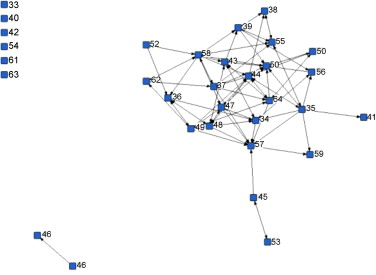
\includegraphics[width=4cm]{wine1.jpg}\\

\medskip

\textbf{2006}\\
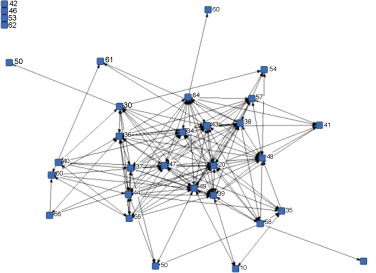
\includegraphics[width=4cm]{wine2.jpg}\\
\tiny{Source:\citet{Giuliani2013}}

\end{columns}

\end{frame}

%------------------------------------------------

\begin{frame}
\frametitle{\insertsection}
\framesubtitle{Observations}

\begin{itemize}
\item Direct observation of the {\color{blue}{interaction among actors}}
\item Used in field research to study relatively {\color{blue}{small groups}}
    \begin{itemize}
    \item non-human primates
    \item attending events (e.g.\ SPRU seminars)
    \item ...
    \end{itemize}
\item Challenges in {\color{red}{observing  multiple actors simultaneously}}
\end{itemize}

\end{frame}

%------------------------------------------------

\begin{frame}
\frametitle{\insertsection}
\framesubtitle{Observations: Example}
\centering
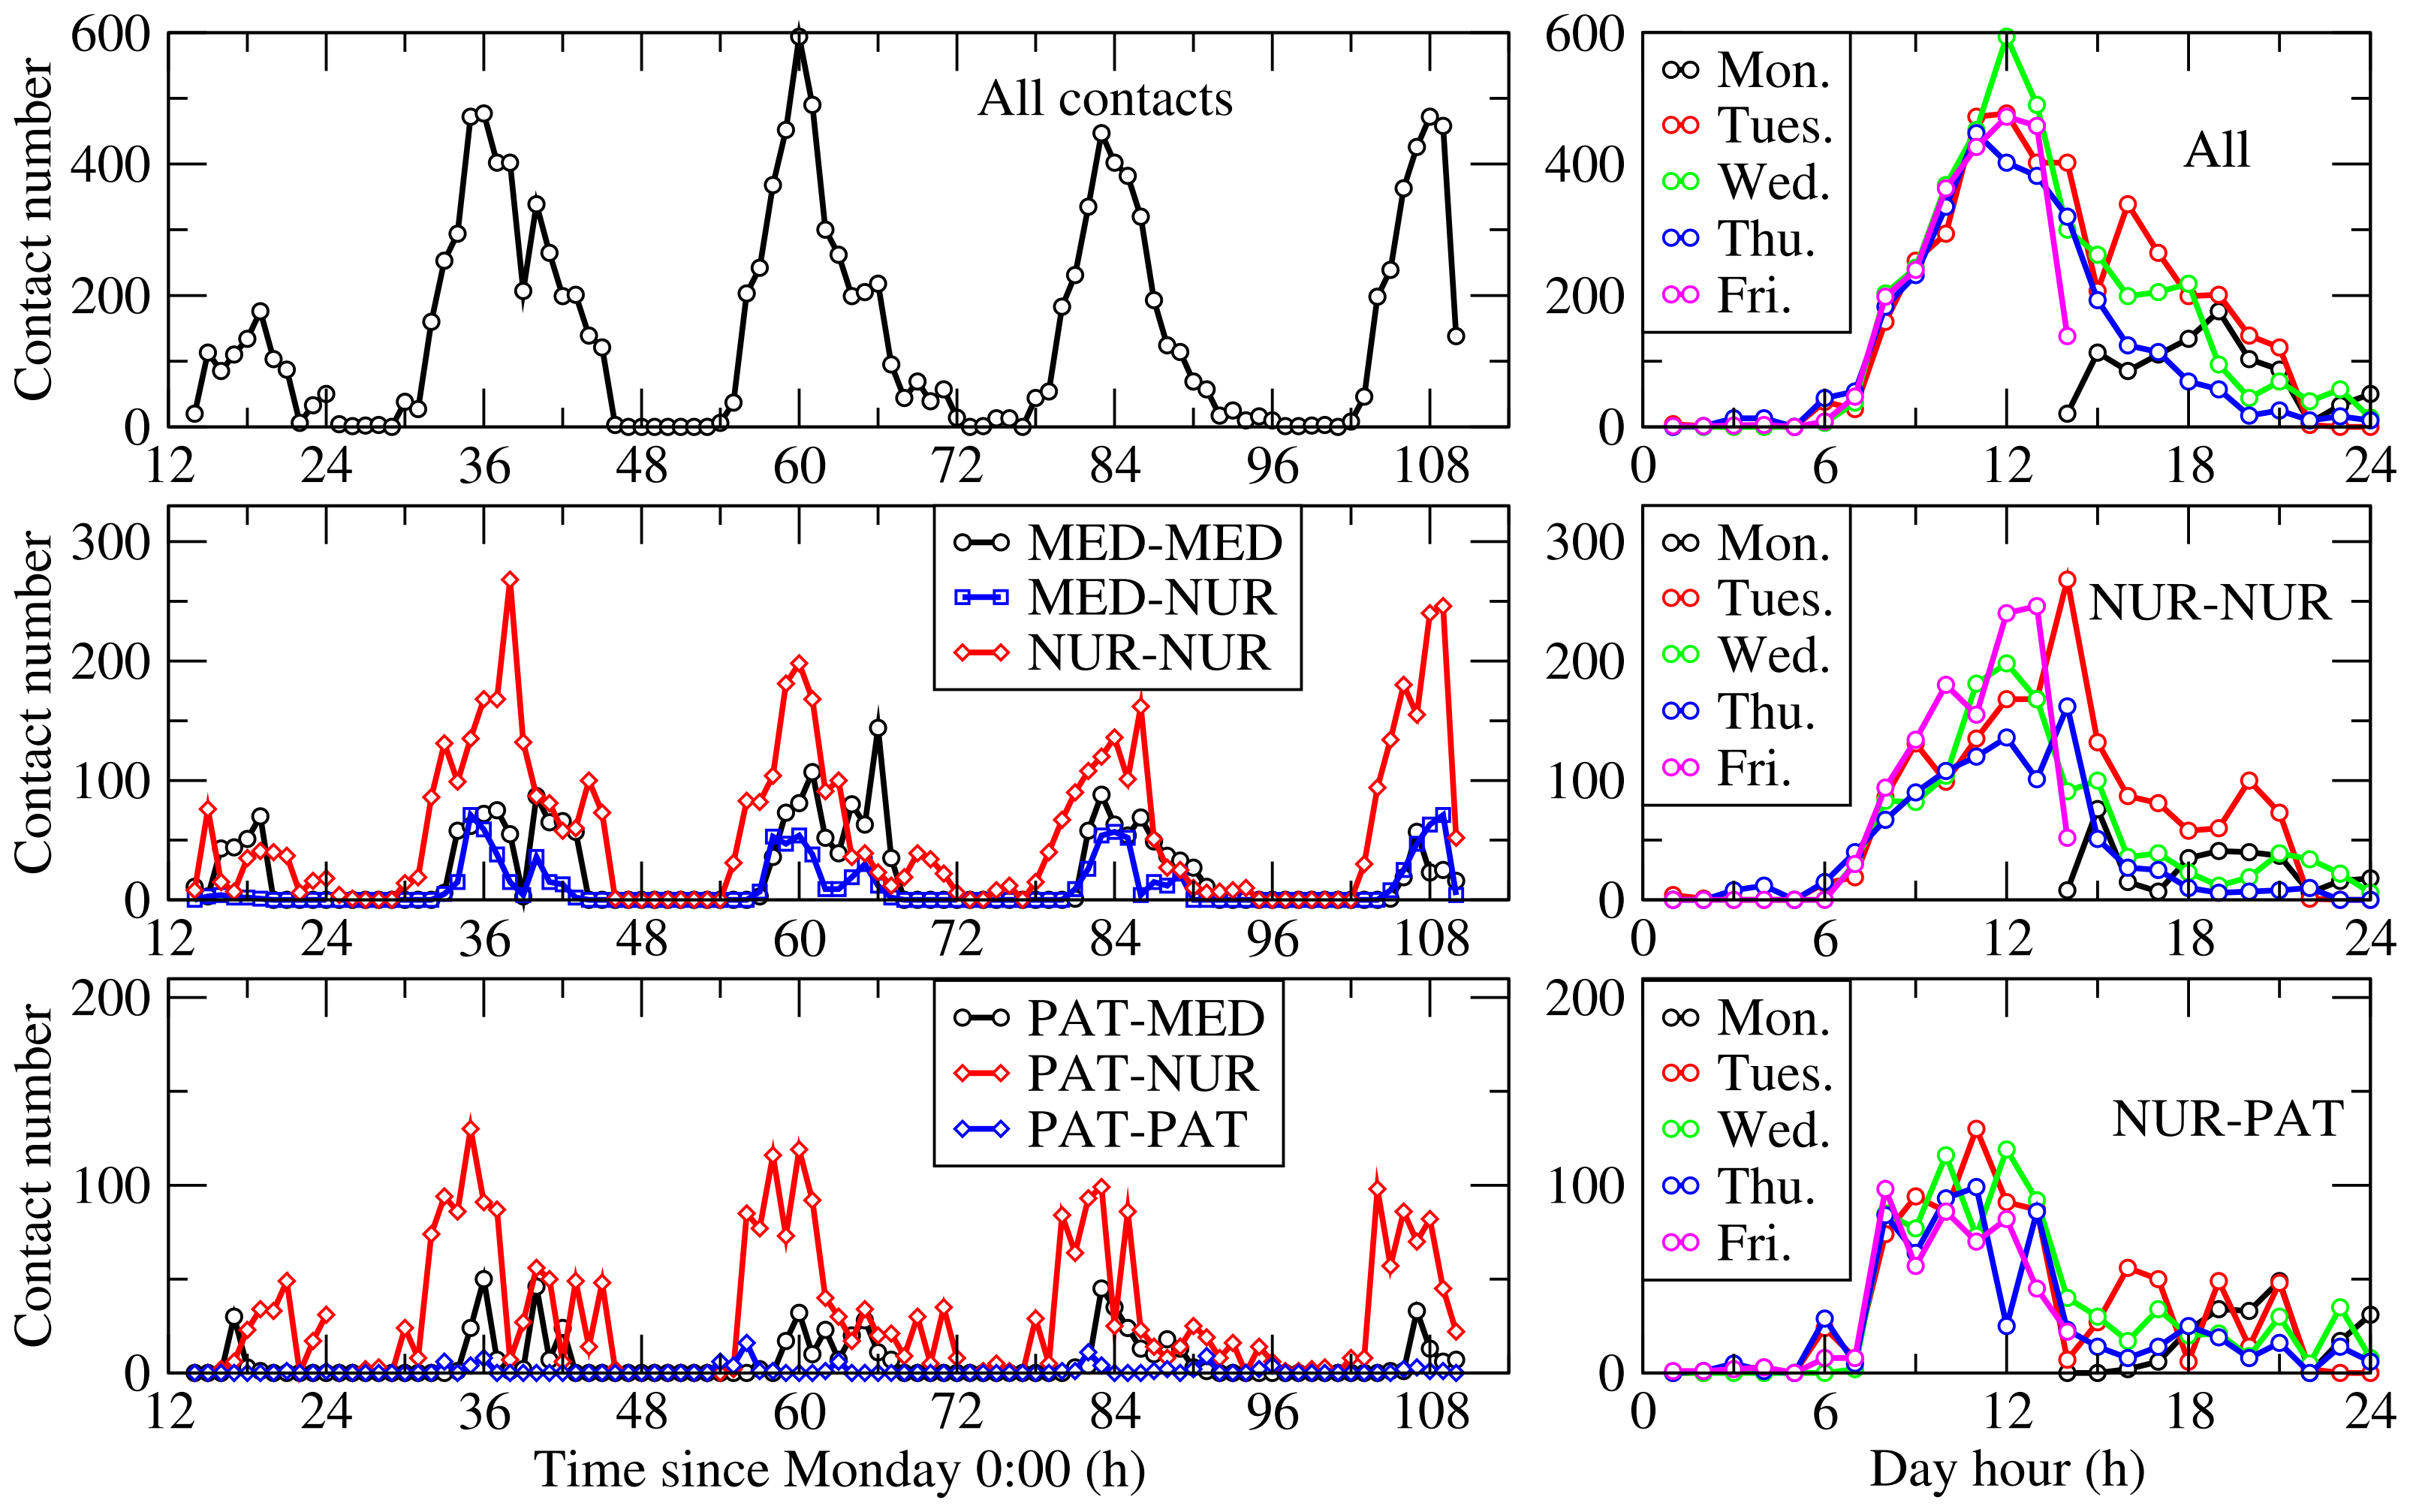
\includegraphics[width=\linewidth,height=0.75\textheight,keepaspectratio]{rfid}\\
\tiny Source: Patient, medical doctor, nurse interactions and infection transmission \citep{Vanhems2013}
\end{frame}

%------------------------------------------------

\begin{frame}
\frametitle{\insertsection}
\framesubtitle{Archival data}

\begin{itemize}
\item {\color{blue}{Records of interactions}} between actors
    \begin{itemize}
    \item Political interactions
    \item Published articles
    \item Collaboration on patents
    \item Citation patterns (publications, patents, scientometrics) 
    \item Bank transactions
    \item ...
    \end{itemize}
   
\item Access to {\color{blue}{large datasets}}
\item Data proxy interactions (validity)
\end{itemize}

\end{frame}

%------------------------------------------------

\begin{frame}
\frametitle{\insertsection}
\framesubtitle{Archival data: Example}
\centering
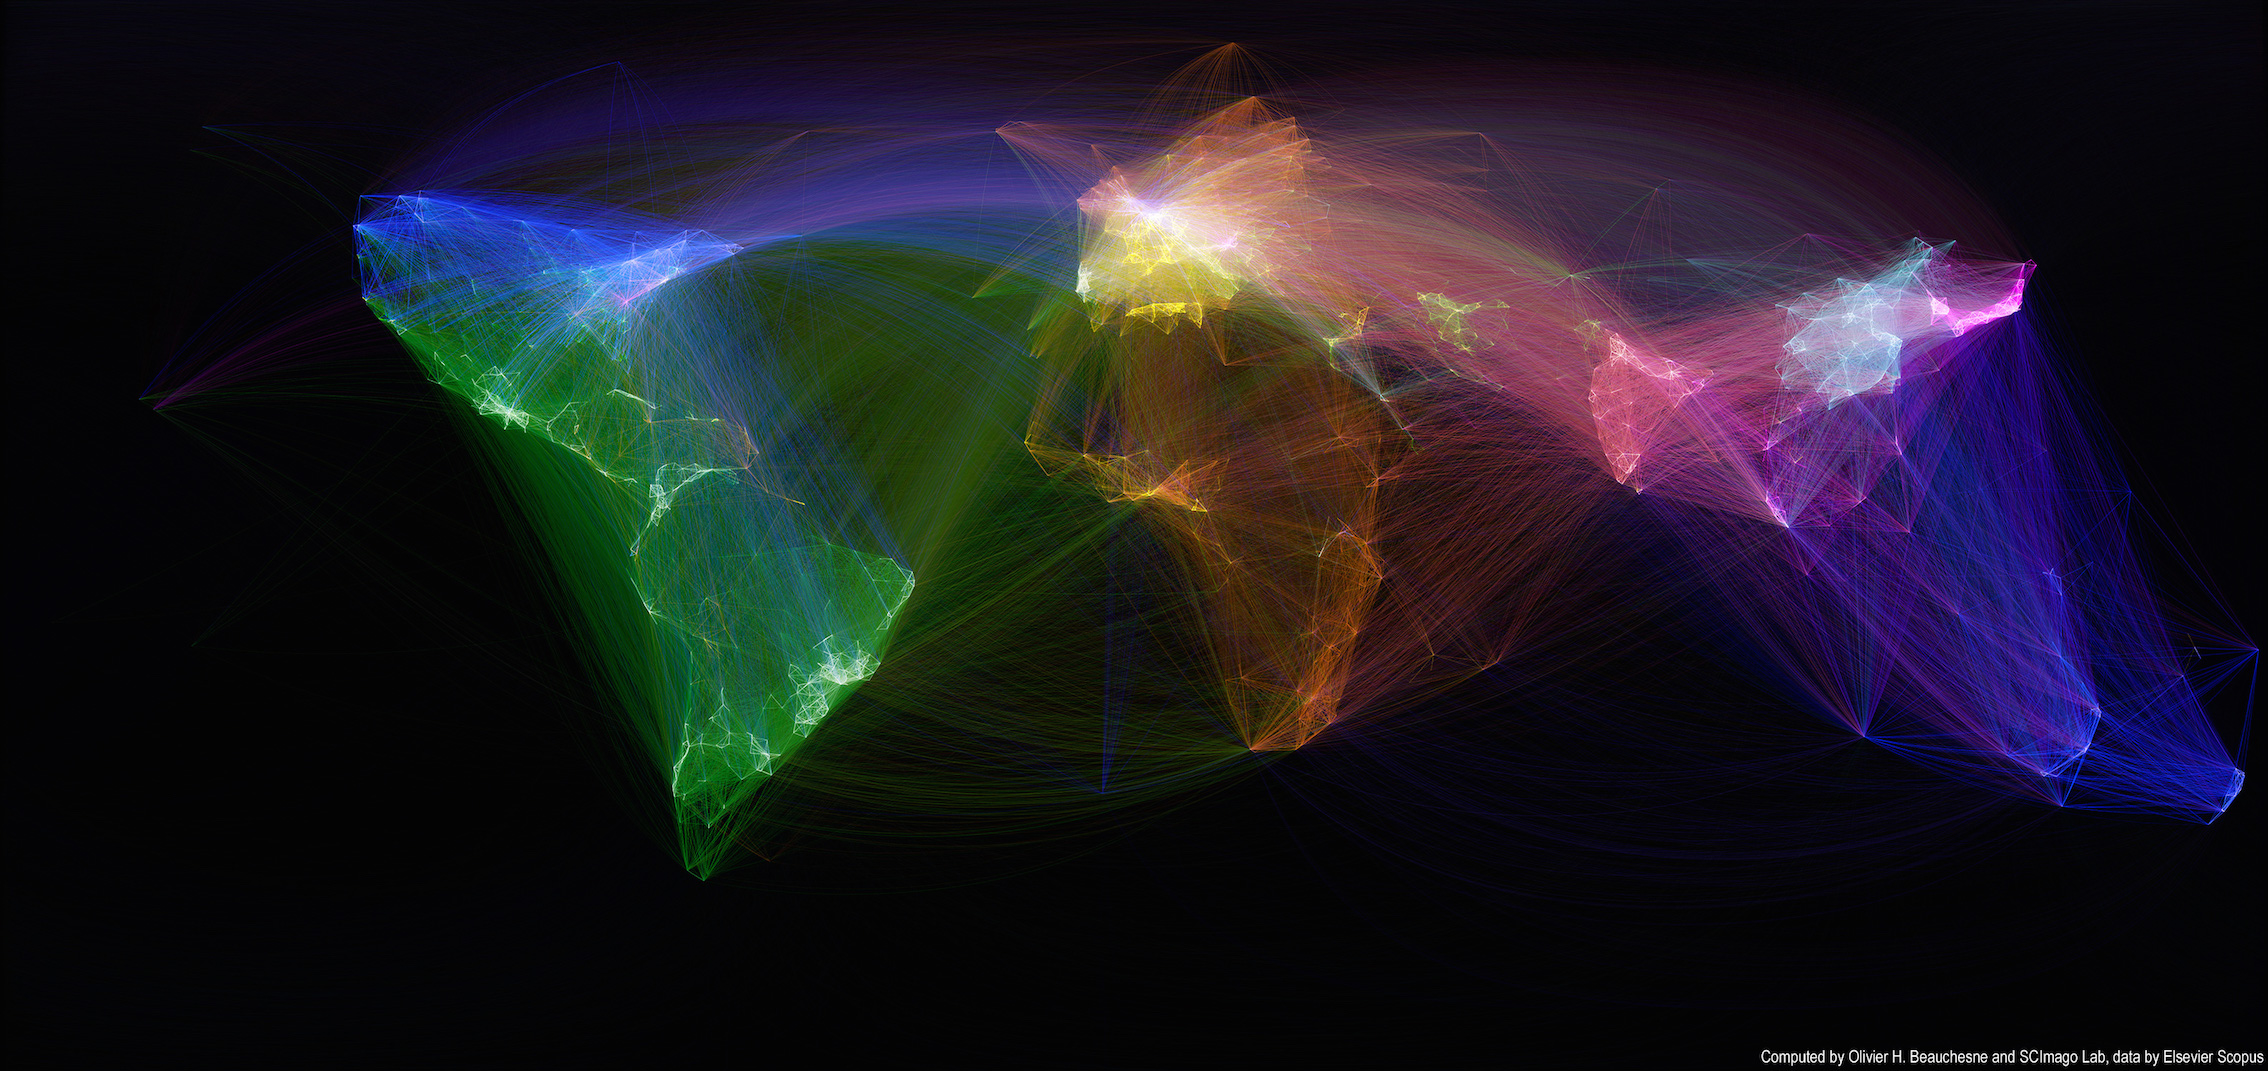
\includegraphics[width=\linewidth,height=0.8\textheight,keepaspectratio]{collaboration}\\     
\tiny Source: Co-authorship at the city level (SCOPUS 2008-2012) [\url{http://olihb.com}]
\end{frame}

%------------------------------------------------

\begin{frame}
\frametitle{\insertsection}
\framesubtitle{Archival data: Example}

\centering
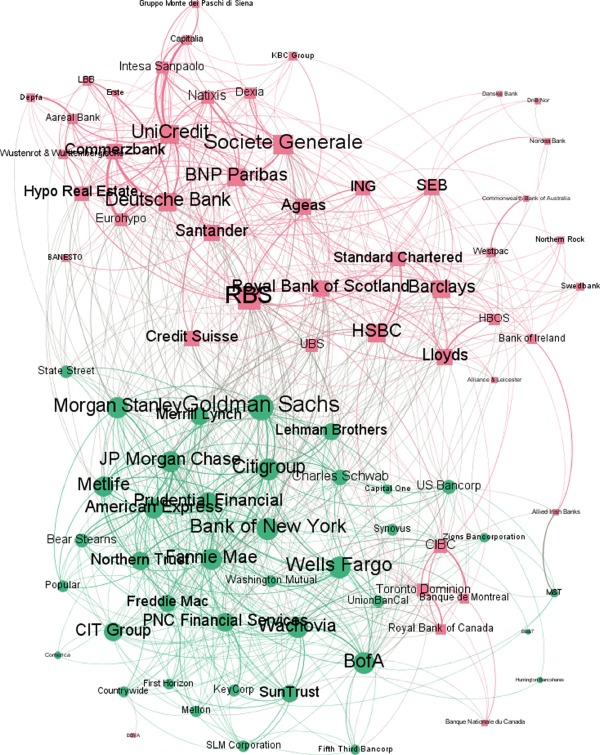
\includegraphics[height = 0.8\textheight]{banking}\\
\tiny{Source: Global banking network in 2006 (banks sharing board members and top management)\citep{Houston2018}}

\end{frame}

%------------------------------------------------






%%=======================================================
% Missing data and measurement challenges
%%=======================================================
\section{Missing data and measurement challenges}

%------------------------------------------------

\bgroup
\setbeamercolor{background canvas}{bg = navyblue}
\begin{frame}[plain]{}
\begin{center}
\color{white}{\Huge\insertsection}
\end{center}
\end{frame}
\egroup

%------------------------------------------------

\begin{frame}
\frametitle{\insertsection}

\begin{columns}[c]
\column{.50\textwidth}
\begin{minipage}[c][0.5\textheight][c]{\linewidth} 
Mechanisms
\begin{itemize}[<+->]
\item Network {\color{blue}{boundary specification}} (non-inclusion of actors or affiliations)
\item Survey {\color{blue}{non-response}}
\item {\color{blue}{Censoring}} by vertex degree (fixed choice design)
\end{itemize}
\end{minipage}


\column{.45\textwidth}
\begin{minipage}[c][0.5\textheight][c]{\linewidth} 
\centering
\only<1>{
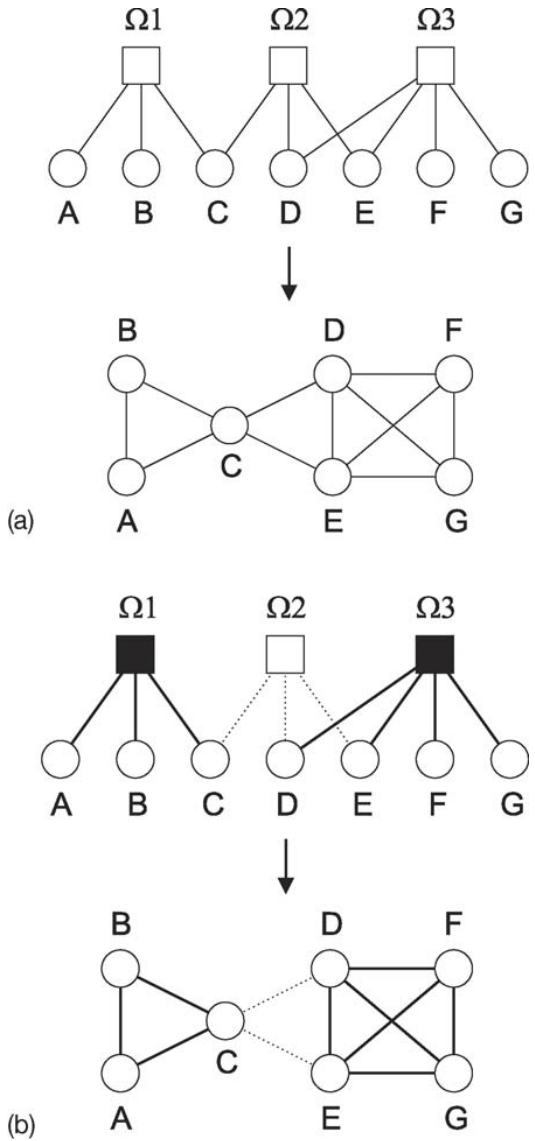
\includegraphics[width=3.5cm]{kossinets_boundary.png}\\
\tiny{Source: Failure to include a context of interaction or affiliation \citep{Kossinets2006}}}

\only<2>{
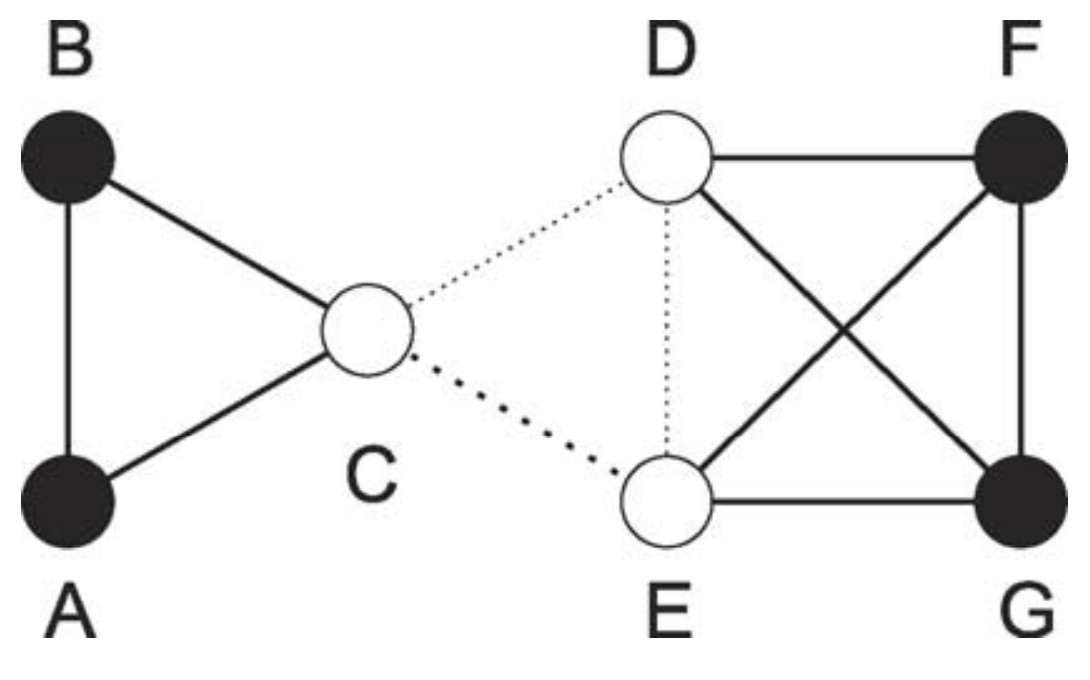
\includegraphics[width=3.5cm]{kossinets_non_response.png}\\
\tiny{Source: Non response of C, D and E links \citep{Kossinets2006}}}

\only<3>{
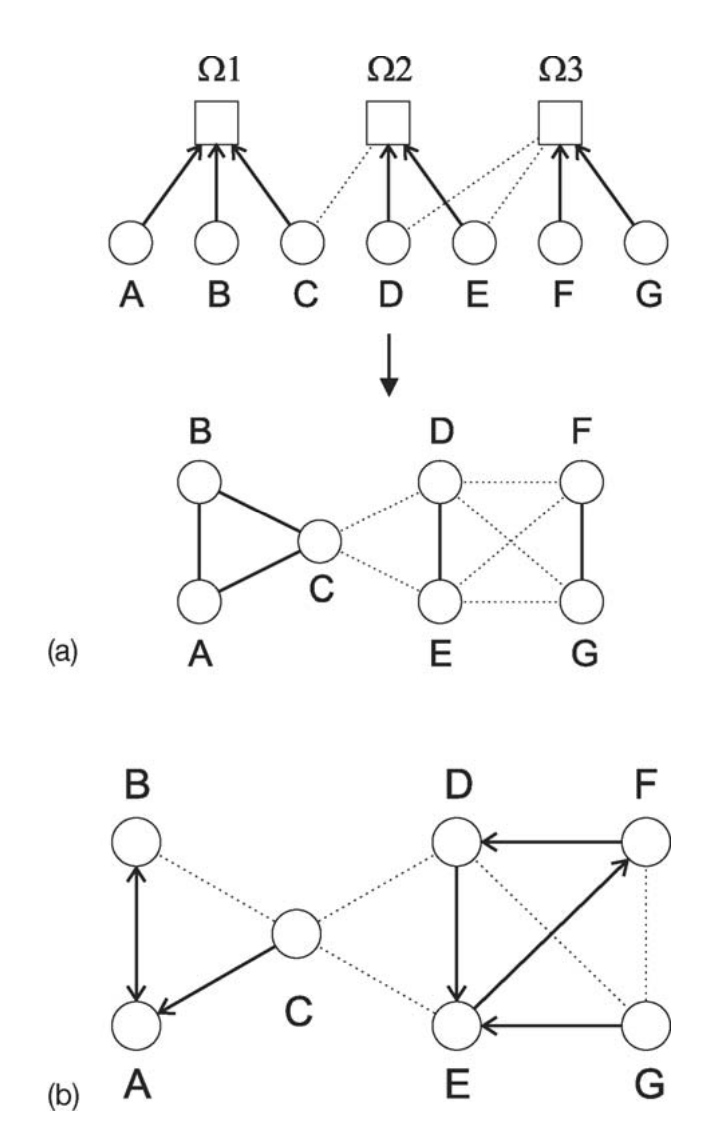
\includegraphics[width=3.5cm]{kossinets_fixed_degree.png}\\
\tiny{Source: Fixed number of nominations of affiliations (a) or acquaintances (b) \citep{Kossinets2006}}}
\end{minipage}

\end{columns}

\end{frame}

%------------------------------------------------

\begin{frame}
\frametitle{\insertsection}

\begin{itemize}
\item {\color{blue}{Accuracy}}
    \begin{itemize}
    \item Respondents are often asked to recall their interactions with other actors
        \begin{itemize}
        \item Organisational network defined on the basis of data collected from individuals
        \item Ego-network and perception of the ties between the peers of the ego
        \item ...
        \end{itemize}    
    \item {\color{dkgreen}{Data triangulation}} (when applicable)
    \end{itemize}

\medskip
\medskip


\item {\color{blue}{Validity}} 
    \begin{itemize}
    \item A measure of a concept is `valid' to the extent that it actually measures what it is intended to measure
    
    \begin{itemize}
    \item Collaboration $\Rightarrow$ co-authorship publications
    \item Friendship $\Rightarrow$ Facebook
    \item Citations in patent data $\Rightarrow$ knowledge flows
    \item ... 
    \end{itemize}
    

    \item {\color{dkgreen}{Construct validity}}: match between measures of concepts and theoretical predictions
    \end{itemize}
    
\end{itemize}

\end{frame}

%------------------------------------------------

\begin{frame}
\frametitle{\insertsection}

\begin{itemize}
    
\item {\color{blue}{Reliability}} 
    \begin{itemize}
    \item A measure of a concepts is `reliable' if repeated measurements produce the same outcome or estimates
    \item Assessing reliability is challenging in the case of social networks (interdependency between observations)
    \item There is evidence that {\color{dkgreen}{complete ranking questionnaires}} tend to produce reliable measures
    \end{itemize}
    
\medskip

\item {\color{blue}{Error}} 
    \begin{itemize}
    \item The error is the difference between the `true' value and the observed value
    \item Fixed choice questionnaires tend to introduce error: it is unlikely that each actor has the same number of ties in a network
    \end{itemize}
    
\end{itemize}

\end{frame}


%------------------------------------------------

\begin{frame}
\frametitle{Design a network data collection}
\framesubtitle{Groupwork}

\begin{columns}[c]

\column{.45\textwidth}
\begin{enumerate}
	\item You will be allocated to a {\color{blue}{group}}
	\item Nominate a {\color{blue}{group leader}} that will be reporting on the activity of the group
	\item Identify a {\color{blue}{network}} about which you would like to collect data and a {\color{blue}{question}} you would like to address with these data
	\item Design a {\color{blue}{data collection approach}} and {\color{blue}{provide a rationale}} for choosing the selected approach
	\item Identify and discuss potential {\color{blue}{challenges}}
\end{enumerate}

\column{.45\textwidth}
\centering
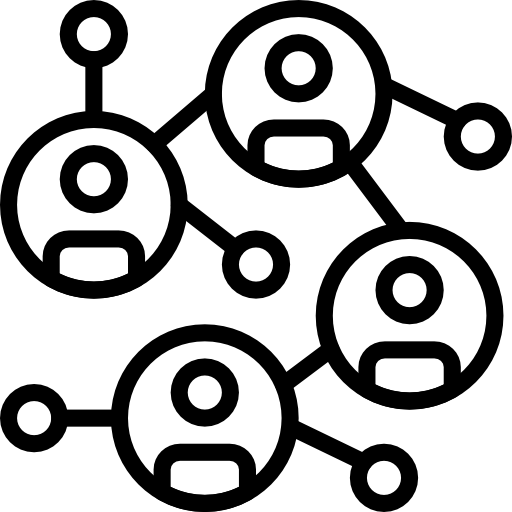
\includegraphics[width=0.8\linewidth]{group_work_team.png}

\end{columns}

\end{frame}

%------------------------------------------------

\begin{frame}
\frametitle{Design a network data collection}
\framesubtitle{Groupwork}


\begin{columns}[c]

\column{.45\textwidth}
\begin{enumerate}
	\item You will be allocated to a {\color{blue}{group}}
	\item Nominate a {\color{blue}{group leader}} that will be reporting on the activity of the group
	\item Identify a {\color{blue}{network}} about which you would like to collect data and a {\color{blue}{question}} you would like to address with these data
	\item Design a {\color{blue}{data collection approach}} and {\color{blue}{provide a rationale}} for choosing the selected approach
	\item Identify and discuss potential {\color{blue}{challenges}}
\end{enumerate}

\column{.45\textwidth}
\centering
\small
\begin{table}
\begin{tabular}{ll}
\toprule
Group 1 & Akanksha \\
		& Belen \\
		& Ross \\
		& Maria\\
		& Ayesha\\
\\
Group 2 & Charunan \\
		& Oscar \\
		& Hiroki \\
		& Saradha\\
\\
Group 3 & Anas \\
		& Ananya \\
		& Evi \\
		& Perizat \\
		& Daniela \\
\\
Group 4 & Samuel \\
		& Jongho \\
		& America \\
		& Noemie \\
\\
Group 5 & Johanna \\
		& Hatty \\
		& Poojani \\
		& Tanya \\
\bottomrule
\end{tabular}
\end{table}

\end{columns}

\end{frame}





%%=======================================================
%	Next time ...
%%=======================================================
\section*{Next time ...}
%------------------------------------------------

\bgroup
\setbeamercolor{background canvas}{bg = navyblue}
\begin{frame}[plain]{}
\begin{center}
\color{white}{\Huge\insertsection}
\end{center}
\end{frame}
\egroup

%------------------------------------------------

\begin{frame}
\frametitle{\insertsection}

\begin{itemize}
\item 	\textbf{Seminar: Network data collection}
	\begin{itemize}
	\item Importa data in R
	\item Network file formats 
	\item How to import and manipulate network data in igraph
	\end{itemize}	
	
\medskip
\medskip
\item 	\textbf{Lecture: Descriptive network analysis A}
	\begin{itemize}
	\item Network measures at the level of the whole network
	\end{itemize}		

\end{itemize}

\end{frame}

%------------------------------------------------






%=======================================================
%	Questions
%=======================================================
\bgroup
\setbeamercolor{background canvas}{bg = orange}
\begin{frame}[plain]{}
\begin{center}
\color{white}{\Huge Questions}
\end{center}
\end{frame}
\egroup







%=======================================================
%	References
%=======================================================
\begin{frame}[allowframebreaks]
\frametitle{References}
\tiny
\bibliographystyle{apalike}
\bibliography{references.bib}
\end{frame}
%------------------------------------------------













\end{document}